%Rule for 71 characters
%2345678901234567890123456789012345678901234567890123456789012345678901

\chapter{The Virtual Observatory} % (fold)
\label{intro_vo}

% \lourdes{Coherencia: buscar ... y quitar o cambiar por et cetera.}
% \lourdes{Coherencia: cambiar et cetera por etcetera.}

% One of the most important achievements of modern astronomy is the %
% digitisation of many relevant datasets, either by scanning old
% photographic plates, or by directly using CCDs or other electronic
% and
% computerised means for data collection. Many archives are available
% which provide astronomers with lots of information without having to
% point themselves a telescope to the sky.
% 
% However, the use of archives brings its new share of problems:
% 
% \begin{description}
% 	\item[Growing list of archives] With new instruments bringing
% 	their own archives, each year a score of new archives joins the
% 	wealth of information available to astronomers. Astronomers,
% 	or software tools, must be notified of the release of
% 	a new archives, and in many cases software would need upgrading
% 	in order to operate with new archives.
% 	
% 	\item[Archive heterogeneity] As each archive is developed by the
% 	team responsible for the corresponding instrument development,
% 	dataset storage, query, and retrieval are created differently for
% 	each instrument or telescope, leading to a strong heterogeneity
% 	both between data products and query methods. Different query
% 	codes have to be written in order to deal with 
% 	
% 	\item[Terabyte-class archives] Archives are growing exponentially
% 	larger, because even when old archives provide a linear storage
% 	rate, new archives provide much larger data rates per day, as
% 	sensitivity and pixel resolutions increase as per Moore's
% 	Law.
% \end{description}

\invisiblenote{
	vir•tu•al |ˈvər CH oōəl| 
	adjective 
	almost or nearly as described, but not completely or according to strict definition : 
	the virtual absence of border controls. 
	• Computing not physically existing as such but made by software to appear to do 
	so : a virtual computer. See also VIRTUAL REALITY . 
	• Optics relating to the points at which rays would meet if produced backward. 
	• Physics denoting particles or interactions with extremely short lifetimes and 
	(owing to the uncertainty principle) indefinitely great energies, postulated as 
	intermediates in some processes.

ob•serv•a•to•ry |əbˈzərvəˌtôrē| 
noun ( pl. -ries) 
a room or building housing an astronomical telescope or 
other scientific equipment for the study of natural 
phenomena. 
• a position or building affording an extensive view. 
}

\attributedquote{
	\dictionarydef
	{virtual}
	{adjective}
	{
		\begin{itemize}
			\item almost or nearly as described, but not completely
			or according to strict definition: 
			\emph{the virtual absence of border controls}.
			
			\item \textsf{Computing} not physically existing as
			such but made by software to appear to do 
			so: \emph{a virtual computer}.
		\end{itemize}
	}
	\dictionarydef
	{observatory}
	{noun}
	{
		\begin{itemize}
			\item a room or building housing an astronomical
			telescope or  other scientific equipment for the study
			of natural phenomena.
			
			\item a position or building affording an extensive
			view. 
		\end{itemize}
	}
}
{The New Oxford American Dictionary, \emph{2nd Edition}}


	
% section the_vo_and_archival_issues (fold)
\section[The VO: solving astronomical archival issues]
[The VO: solving astronomical archival issues]
{The Virtual Observatory: solving astronomical archival issues}
\label{sec:the_vo_and_archival_issues}
	
	In the previous chapter the current status of multi-wavelength,
	archive based astronomy was laid as well as the problems
	arising when dealing with the increasing number of data
	archives available to the astronomical community, and with the
	increasing sizes for each data unit. Additionally, these data
	units must be combined in order to obtain a multiwavelength
	view of our universe.
	
	 As the archives are already distributed across the world, the
	solution must be network-enabled, and must be as modular as
	possible, so that different data providers and astronomical
	tool developers can work independently, and rely on common
	interfaces. A Service Oriented Architecture (SOA), where data
	providers create web-services, and tool developers use
	web-services interfaces to query them fits that description,
	and allows reuse of already existing and deployed technology.
	
	 It must be noted that astronomical data reduction for large
	instruments is a highly specialised task, and that data
	reduction techniques are improved when knowledge about the
	underlying processes (astrophysical and observational)
	improves. This specialisation, and the long term variability of
	reduction techniques, makes unfeasible the centralisation of
	astrophysical archives.
	
	 In any case, those services must be oriented to astrophysics,
	and responses must include metadata describing the
	peculiarities of each data set. \invisiblenote{The choice of
	SOA makes XML the perfect language for holding the metadata for
	astronomical data sets.} Lastly, in order for applications to
	find out both existing and new services and data sets, a common
	service registry is needed for VO applications to find out
	suitable services and data sets.
	
	 Jim Gray and Alexander Szalay, in ``The World-Wide
	Telescope''~\cite{2001Sci...293.2037S}, were among the first to
	outline such a system, which is called the Virtual Observatory
	(VO). In that paper, they analysed the already mentioned
	exponential trends of instrumental data output and archived
	data holdings increase, and noticed the not equally growing
	gain in astrophysical insight as an unmistakable sign that
	astronomers were not being able to cope with the new
	data-driven situation, and needed new tools to get the most of
	the extremely large datasets now available to them.
	
	 An example of a widely used, very large astronomical dataset
	is the already mentioned SDSS. In its latest release (DR7), the
	SDSS consists of more than 15~TB of image data, plus more than
	25~TB of ancillary data, and 18~TB of catalogue data. There is
	not enough bandwidth at the SDSS or at the different research
	institutions to transfer all the data to all researches which
	would like to use the SDSS. And in the future, surveying
	telescope such as the Large Synoptic Surveying Telescope (LSST)
	will produce and process around 7~TB of raw data per night.
	
	 Exploiting this ever-increasing amount of data is only
	feasible by scientific-case guided data selection, together
	with automated data mining techniques. But for that to be
	performed in a fully automated way, data archives and data
	analysis tools must become interoperable.

	% \lourdes{Reordenar conforme capítulo.}

	For achieving the interoperability we will need, as stated by
	F.~Genova in her ``Interoperability''
	article~\cite{2002ASPC..281...41G}:
	
	\begin{itemize}
		\item common data formats;
		
		 \item common data access protocols; and
		
		 \item common data models for the same type of
		observations, as independent as possible of the generation
		of the dataset, so that data from very different
		observatories and instruments can be combined.
	\end{itemize}
	
	 In addition, as VO services are distributed across the globe,
	and can be deployed anywhere, anytime, one or several services
	registries are needed, so that users can find and discover new
	services.
	
	 But for those common formats, protocols and data model to
	become truly compatible an standardisation body is needed. In
	the VO, that body is the International Virtual Observatory
	Alliance.
	
	 In the next sections we will see how the VO achieves archive
	interoperability, which mechanisms provides for minimising
	local data processing as much as possible, and what is the high
	level organisation of the IVOA.
% section the_vo_and_archival_issues (end)


\section{VO architecture and philosophy} % (fold)
\label{sec:vo_architecture}

	In Gray and Szalay's paper~\cite{2001Sci...293.2037S}, the
	stated philosophy for the VO is that of an
	e-infrastructure\footnote{The \emph{e} in e-infrastructure does
	not stand for \emph{electronic}, but for \emph{enhanced}, as in
	\emph{e-Science}, or \emph{enhanced science}. The enhancement
	is produced by means of the massive use of networked resources,
	such as data grids, computation grids, distributed storage, et
	cetera, which conform the \emph{e-infrastructure}.} which makes
	all astronomical data in the world available for astronomers as
	if they were in their own desktop, without the limitations of
	desktop computing.
	
	 For many large datasets the user should not deal with the data
	directly, as the data transport time for many modern datasets
	is not negligible, and the data producer's infrastructure can
	be better suited for remote processing. In time, remote
	processing has to become commonplace, as it will become the
	only solution to let users ask questions to datasets much
	larger than typical workstation can manipulate, avoiding
	network bottlenecks at the same time.
	
	 In any case, sufficient metadata must be provided so that
	astronomers do not need to download data to see if they can be
	useful or interesting, and perform instead a suitable selection
	of datasets based on metadata. In particular, data quality
	assessment through metadata inspection and evaluation allows
	astronomers not to retrieve, for instance, low resolution
	datasets if they need precise astrometric measurements, while
	other astronomers interested on obtaining upper limits of an
	object's emissions might find them useful.

%	\lourdes{redactar el párrafo anterior para que no indique que
%	se usen datos faulty, sino quizá upper limits o similares o not
%	fully calibrated}

	How is that vision actually implemented?
	Figure~\ref{fig:fig_VOArch} portraits a simplified,
	all-encompassing vision of the Virtual Observatory. In that
	figure we see the Virtual Observatory from the lowest level
	supporting implementation (network cabling, routers, storage
	media, et cetera; what is usually known as \emph{the iron}), to
	base internet protocols, and grid computing middleware, to VO
	services and protocols implemented on top of that
	infrastructure, and applications using both services and
	protocols to present the user with a unified interface.

\newcommand{\voarchitecturenoteurl}[0]
{http://www.ivoa.net/Documents/Notes/IVOArch/IVOArch-20040615.html}
	\begin{figure}[tbp]
		\centering
			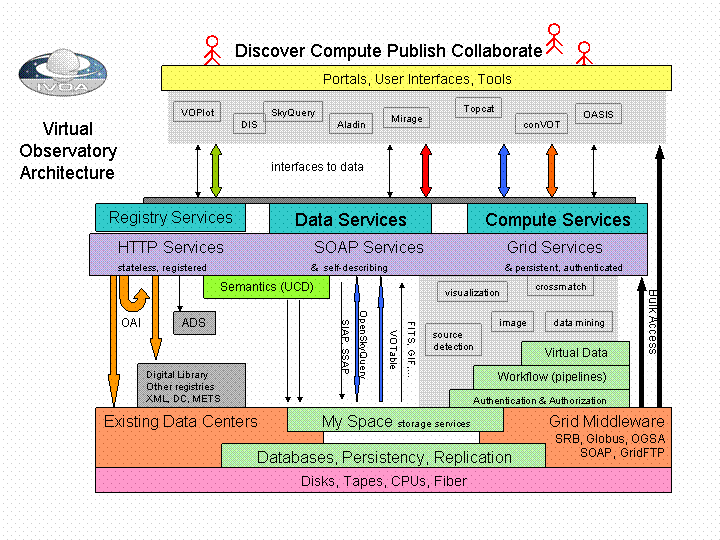
\includegraphics[width=\columnwidth]
			{fig/VO_Architecture.png}
		\caption[Virtual Observatory architectural overview]
		{
			Architecture of the Virtual Observatory, seen from the
			low level implementation (bottom) to the user (top).
			Users perform high-level activities, such as
			computations, data discovery, data mining, and even
			publishing into the VO by means of applications,
			scripting tools, or web portals. Applications
			communicate with the VO by means of IVOA approved
			protocols to access the service Registry, Data Services
			to retrieve astronomical images, spectra or, in the
			near future, complex table access to astronomical
			databases. Computing Services are needed for those
			computations which are costly to perform locally due to
			bandwidth or processor requirements. Registries
			communicate with each other via the Open Archive
			Initiative (OAI) harvesting protocols, to ensure that
			registry changes propagate from each registry to the
			rest. Registries are queried through SOAP-based
			protocols, to ensure compatibility with other OAI
			registries, while the remaining VO protocols use simple
			HTTP GET (REST-ful) interfaces. From the IVOA Virtual
			Observatory Architecture Overview diagram,
			\url{\voarchitecturenoteurl}.
			% \todoinline{Recreate simplified diagram.}
		}
		\label{fig:fig_VOArch}
	\end{figure}

%	Figure~\ref{}, on the other hand, provides a mind map of the
%	Virtual Observatory concepts. The

	 It is legitimate to ask how far is the Virtual Observatory
	today from being completely transparent to the user. The answer
	to that is that there are several factors which make the
	Virtual Observatory still a separate environment for
	astronomical research:

	\begin{itemize}
		\item VO applications and portal are still unknown to many
		astronomical users, including some data providers. The
		different VO groups are making an effort in the
		dissemination of the VO concept, both for astronomical
		users and data providers. Many different workshops and
		schools are being promoted in order to reach users and
		providers.
		
		 \item Many interesting datasets are still not available
		via the VO. The NVO and the Euro-VO projects, are
		developing tools to make data publishing easier for small
		research groups. However, they demand a high level of
		computing expertise in the domain of networking, web
		services technologies, XML, and of the inner workings of
		the VO. Besides, a commitment to maintain the archive
		operational in the long term means the research group has
		to keep storage and network resources with a high level of
		availability. This makes it difficult for those small
		groups to become data publishers if they do not deploy a
		complete archive.
		
		 \item Many different useful tools for astronomers predate
		the Internet era, with many legacy tools unable to access
		Virtual Observatory datasets.
	\end{itemize}

%	This thesis tries to address these three concerns, in the
%	framework of radio astronomy. In this thesis:
%
%	\begin{itemize}
%		\item We present the VO both from the astronomical and
%		computer science sides, so that more developers can
%		contribute to the VO, and more astronomers are made aware
%		of its posibilities.
%		
%		 \item We provide a framework for radio astronomical
%		observation characterisation and data publishing, which has
%		actually been used for the development of the IRAM~30m and
%		Robledo's DSS-63 archive.
%		
%		 \item We follow different strategies for making legacy
%		astronomical applications aware of the VO, and able to use
%		VO datasets.
%	\end{itemize}

% 	\subsection{The VO protocol stack} % (fold)
% 	\label{sub:the_vo_protocol_stack}
% 
% 	\setlength{\epigraphwidth}{0.66\columnwidth}
% 
% 	\epigraph{
% 		Any problem in computer science can be solved with another
% 		level of indirection... but that will usually create another
% 		problem.
% 	}
% 	{\textsc{David Wheeler}, as quoted by \textsc{Butler Lampson}}
% 	
% 		The architecture of the VO can be seen in a simplified way by
% 		means of the OSI diagram. Figure~\ref{} shows the typical
% 		depiction of a network protocol stack, where different
% 		machines communicate between them conceptually at the same
% 		level, while the actual communication is from the upper part
% 		of the stack to the lower part, with results from the lower
% 		parts to the upper parts.
% 		
% 		 In that view, each layer calls services in the lower layer,
% 		so that higher-level capabilities (rendering of web pages, for
% 		instance) rely on a protocol layer (HTTP), which relies on a
% 		transport protocol (TCP), relying on a network routing
% 		protocol (IP), which relies on data link and physical
% 		technologies, such as wired or wireless networking over
% 		Ethernet, LocalTalk, Token Ring, or any other networking
% 		settings.
% 		
% 		 In the case of the VO, interchanges happen at the Application
% 		and Presentation layers, as all of IVOA protocols are based on
% 		top of HTTP and HTTPS (some of them can use other protocols,
% 		but HTTP/S is a requirement)
% 	
% 	% subsection the_vo_protocol_stack (end)

% section vo_architecture (end)

% \todoblock{
% 	When talking about VO architecture, present the VO from the 
% 	point of view of:
% 
% 	\begin{itemize}
% 		\item the user [done]
% 		\item the VO application (developer) [done]
% 		\item the VO service (developer)
% 		\item the data centre/scientist wishing to publish on VO
% 		\item the infrastructure provider
% 	\end{itemize}
% 
% - VO architecture
% 
% 	- Layers
% 
% 	- Agents
% 
% 	- SOA (sort of...)
% 
% 		- Services and Clients
% 
% 			- SOAP
% 
% 			- REST
% 
% 			- Common Execution Architecture
% 
% 	- Local interoperability: RPC, XML-RPC
% 
% 		- Meta-data preservation
% 
% 	- Similarities and differences with Grid and Data Grid
% 
% 	\todo{
% 		Talk about what would be a VO Service Bus for applications
% 	}
% }

	\section{VO data formats} % (fold)
	\label{sub:vo_data_formats}

		\invisiblenote{The key word to the Virtual Observatory, and
		similar e-Science efforts, is \emph{interoperability}. Only
		if all applications can use data from all archives can
		those archives' data become truly interoperable, and for
		that one of the most important pieces is a common data
		format. Françoise Genova wrote a very illustrative article
		on interoperability within
		astronomy~\cite{2002ASPC..281...41G}, stressing the three
		legs on which interoperability relies: data formats, data
		access, and data semantics, expressed in data models.}
		
		 One of the three key aspects of interoperability, as we
		have seen,is data formats. If applications do not know how
		to operate with the files containing the data relevant to
		them it does not matter if data was compliant with a given
		data model, or if it was accessible from a common access
		protocol.

		\subsection{The FITS data format} % (fold)
		\label{ssub:the_fits_data_format}

			It was radio astronomy, in particular radio
			interferometry, which started with the need for a
			common data format. Interferometric observations
			provide astronomical images by means of the inverse
			Fourier Transform of a sparsely sampled 2D Fourier
			expansion. As reconstruction algorithms needed
			expensive equipment and long processing times to
			provide the images, and later additional cleaning
			algorithms had to be run, it made sense to create a
			common data format which allowed for the interchange of
			scientific grade astronomical image (and visibilities)
			products, so that data could be moved to powerful
			enough computers. That format is the Flexible Image
			Transport System (FITS), created in the late seventies,
			and finally published in
			1981~\cite{1981A&AS...44..363W}.
			\invisiblenote{The reader
			can find more detail about the FITS file format in
			appendix~\ref{cha:description_of_the_fits_file_format}.}
			
			 The main benefit from the FITS file format was the
			decoupling of actual instrument data from data about
			the instrument and observation setup (metadata). Data
			resided in image or table extensions, while metadata
			was expressed in the form of ASCII headers, such as
			\texttt{TELESCOP} for specifying an observatory, or
			\texttt{INSTRUME} for specifying a particular
			instrument within that observatory.
			
			 However, the FITS file format, over the years,
			developed its own share of problems:

			\begin{itemize}
				\item Only a small core vocabulary is defined.
				Additional headers can be used in non-standard
				ways. The IAU Working Group in charge of the file
				format does not mandate particular keywords, or
				proposes best practices for FITS archival.
				
				 \item Multiplicity of \emph{de facto} per
				instrument and per package FITS standards: for
				instance, the AIPS++ radio interferometry reduction
				program uses a convention called
				FITS-IDI~\cite{2000aips.memo..102F} (FITS
				Interferometry Data Interchange), while AIPS, its
				ancestor, uses the UVFITS convention. On the single
				dish side, IRAM uses the IMB-FITS
				format~\cite{MudPolHat0512Multi-Beam}, while others
				use the SDFITS~\cite{2000ASPC..216..243G} (Single
				Dish FITS) convention. That means that observation
				metadata, such as calibration curves, tipping
				measurements (skydips), et cetera, could be
				included with the file as additional tables or not,
				depending on observatory, and some times depending
				on the instrument.
				
				 \item FITS is not an appropriate file format for
				archival purposes. There is a flat header for all
				extensions, and it is physically joined to the
				corresponding metadata. In order to index a FITS
				archive, additional layers have to be applied.
				
				 \item FITS files cannot be streamed on the fly
				from an instrument: given the fact that FITS is
				block oriented (due to its origin as an image
				\emph{transport} format using computer tapes), it
				is very difficult to generate a valid FITS file
				from a continuous stream of data. At most,
				different FITS files can be created for different
				runs of an observation (per scan, or per
				integration), and then written down as a FITS file.
				But a truncated FITS file is very difficult to
				recover without manual tweaking, or to be
				interpreted automatically, apart from the ASCII
				Header part. Conversely, FITS files cannot be read
				sequentially, either, and a FITS file needs to be
				completely read (apart from the Header), in order
				to interpret its data.
				
				 \item There is no way to combine data from
				different instruments, as units and scales are
				specified in a human readable, but not computer
				understandable form.
			\end{itemize}

			The latest \emph{Definition of the Flexible Image
			Transport System (FITS)}
			document~\cite{FITS-Working-Group:2008ty} still
			includes phrases referring to some features of the FITS
			file format as legacy, but used by the earlier
			packages, while new instruments use additional
			mechanisms not compatible with those used by the oldest
			tools. It is not uncommon (or unheard of) needing to
			manually change FITS files, or file generation
			parameters, to make FITS files read from an archive, or
			observed from other instruments, compatible with
			particular tools.
			
			 With all of its shortcomings, the fact that FITS files
			allow for the storage of images, spectra, and other
			tables, with additional metadata describing those data
			products, has been enormously beneficial for the
			astronomical community, as it has made data
			distribution and tools development considerably easier.
			
			 Besides, the main capabilities of the FITS file
			format, which make it the most successful data format
			in astronomy to date, and is still in wide use today
			(to the point of being an integral part of the VO), are
			the following:

		\newcommand{\fitsiourl}[0]
	{http://heasarc.gsfc.nasa.gov/docs/software/fitsio/fitsio.html}
		\newcommand{\nomtamfitsurl}[0]
	{http://heasarc.gsfc.nasa.gov/docs/heasarc/fits/java/v0.9/}
		\newcommand{\pyfitsurl}[0]
	{http://www.stsci.edu/resources/software_hardware/pyfits}

			\begin{description}
				\item[Flexibility] At the same time FITS weakness
				and strength, the format flexibility\footnote{FITS
				flexibility is based on the ability of FITS files
				of containing an arbitrary number of
				multidimensional arrays, each one with its own FITS
				headers for describing its content. However, it is
				not possible to specify whether different arrays
				are related in any way. For instance, if one of the
				arrays corresponds to a reduced spectrum, and
				another one corresponds to sky spectrum which has
				been subtracted, the only way to know it would be
				by manual inspection of the FITS file.} has allowed
				it to respond to the changing needs in astronomy,
				transporting data both from ground-based and
				space-born optical telescopes' images, radio
				telescope single dish spectra, maps or On-The-Fly
				observations, radio interferometer visibility,
				imaging, and data cubes, optical Fabry-Perot
				interferometer data cubes, Integral Field Units 3D
				spectroscopy, et cetera. The array of different
				telescopes and instruments using the FITS file
				format comprises the entire observational
				community.
				
				 \item[Large availability of support libraries]
				From the beginning, astronomy software developers
				could rely on \texttt{fitsio}\urlnote{\fitsiourl},
				a FITS read and write library with access to the
				full array of capabilities of the FITS data format.
				That library was written in FORTRAN, but soon a
				\texttt{cfitsio} library was released for C/C++
				development. For Java, support is provided by the
				\texttt{nom.tam.fits}\urlnote{\nomtamfitsurl}
				library, and for Python a \texttt{NumPy}-compatible
				\texttt{PyFITS}\urlnote{\pyfitsurl} library exists.
			\end{description}

			There are a large number of archives providing FITS
			files, and for the VO to be successful, and have those
			archives provide VO compatibility, the VO must
			accommodate FITS files.

		% subsection the_fits_data_format (end)

		\subsection{The VOTable} % (fold)
		\label{ssub:the_votable}
		
			Any new data format wishing to achieve the same
			diffusion as FITS needs to keep FITS' main strengths
			---flexibility, and availability of libraries and
			tools---, while addressing most of its shortcomings.
			
			 The VOTable is the main VO data format for the
			interchange both of tabular data, and of metadata
			related to any kind of astronomical data, and has the
			following properties:
			
			\begin{description}
				\item[XML data format] The VOTable is an XML-based
				data format, and as such, it earns a wide
				availability of data writing and consumption
				libraries. XML documents can be queried through the
				XQuery language, or transformed in different kind
				of documents with XML Style-sheet Transformations
				(XSLTs). Plus, XML documents and processors are
				inherently internet-ready, providing mechanisms for
				linking with datasets located anywhere in the
				internet. Prior to the VOTable, different attempts
				at combining XML with FITS files had been
				made~\cite{2000ASPC..216...83O,
				2001ASPC..238..487T}, and other XML-based based
				file formats~\cite{Blackburn:1999fu,
				2000AAS...19711602S} had been devised to replace
				FITS files.
				
				 \item[Namespace support] Stemming from its XML
				origin, VOTables can embed terms from different
				namespaces, thus allowing further flexibility and
				extensibility, without losing the origin and
				semantics of the extension.
				
				 \item[Data and metadata separation] VOTables are
				much more verbose than FITS files ---something
				common to all XML-based data formats---, and
				typical data sizes are bigger. However, the linking
				mechanism allows XML-metadata to be processed and
				queried without having to download the actual
				astronomical data. What is more, particular FITS
				sections can be referenced from any VOTable, so
				that different VOTables can point to the same table
				of a FITS file, or the same VOTable can point to
				different tables of the same FITS file.
				
				 \item[Astronomical and astrophysical semantics]
				VOTables have astronomy specific tags, such as
				coordinate system definitions, but \texttt{FIELD}
				elements can optionally provide \texttt{units}
				attributes, and for the clarification of the
				general kind of information in each field, a
				\texttt{ucd} attribute ---short for Universal
				Content Descriptor, UCD--- can be used. We will see
				that the UCDs provide metadata with semantics which
				come from IVOA defined data models, and that
				additional \texttt{utype} attributes can be used to
				further specify a particular field within a
				particular data model.
				
				 \item[Support for FITS file linking] The VOTable
				can hold data by itself, but the linking mechanisms
				are typically used for providing internet access to
				FITS files.
			\end{description}
			
			Figure~\ref{fig:fig_amiga-vot} shows an example VOTable
			obtained from the AMIGA VO catalog, with the metadata
			for the description of a four column table, with three
			rows returned.
			
			\begin{figure}[tbp]
				\centering
					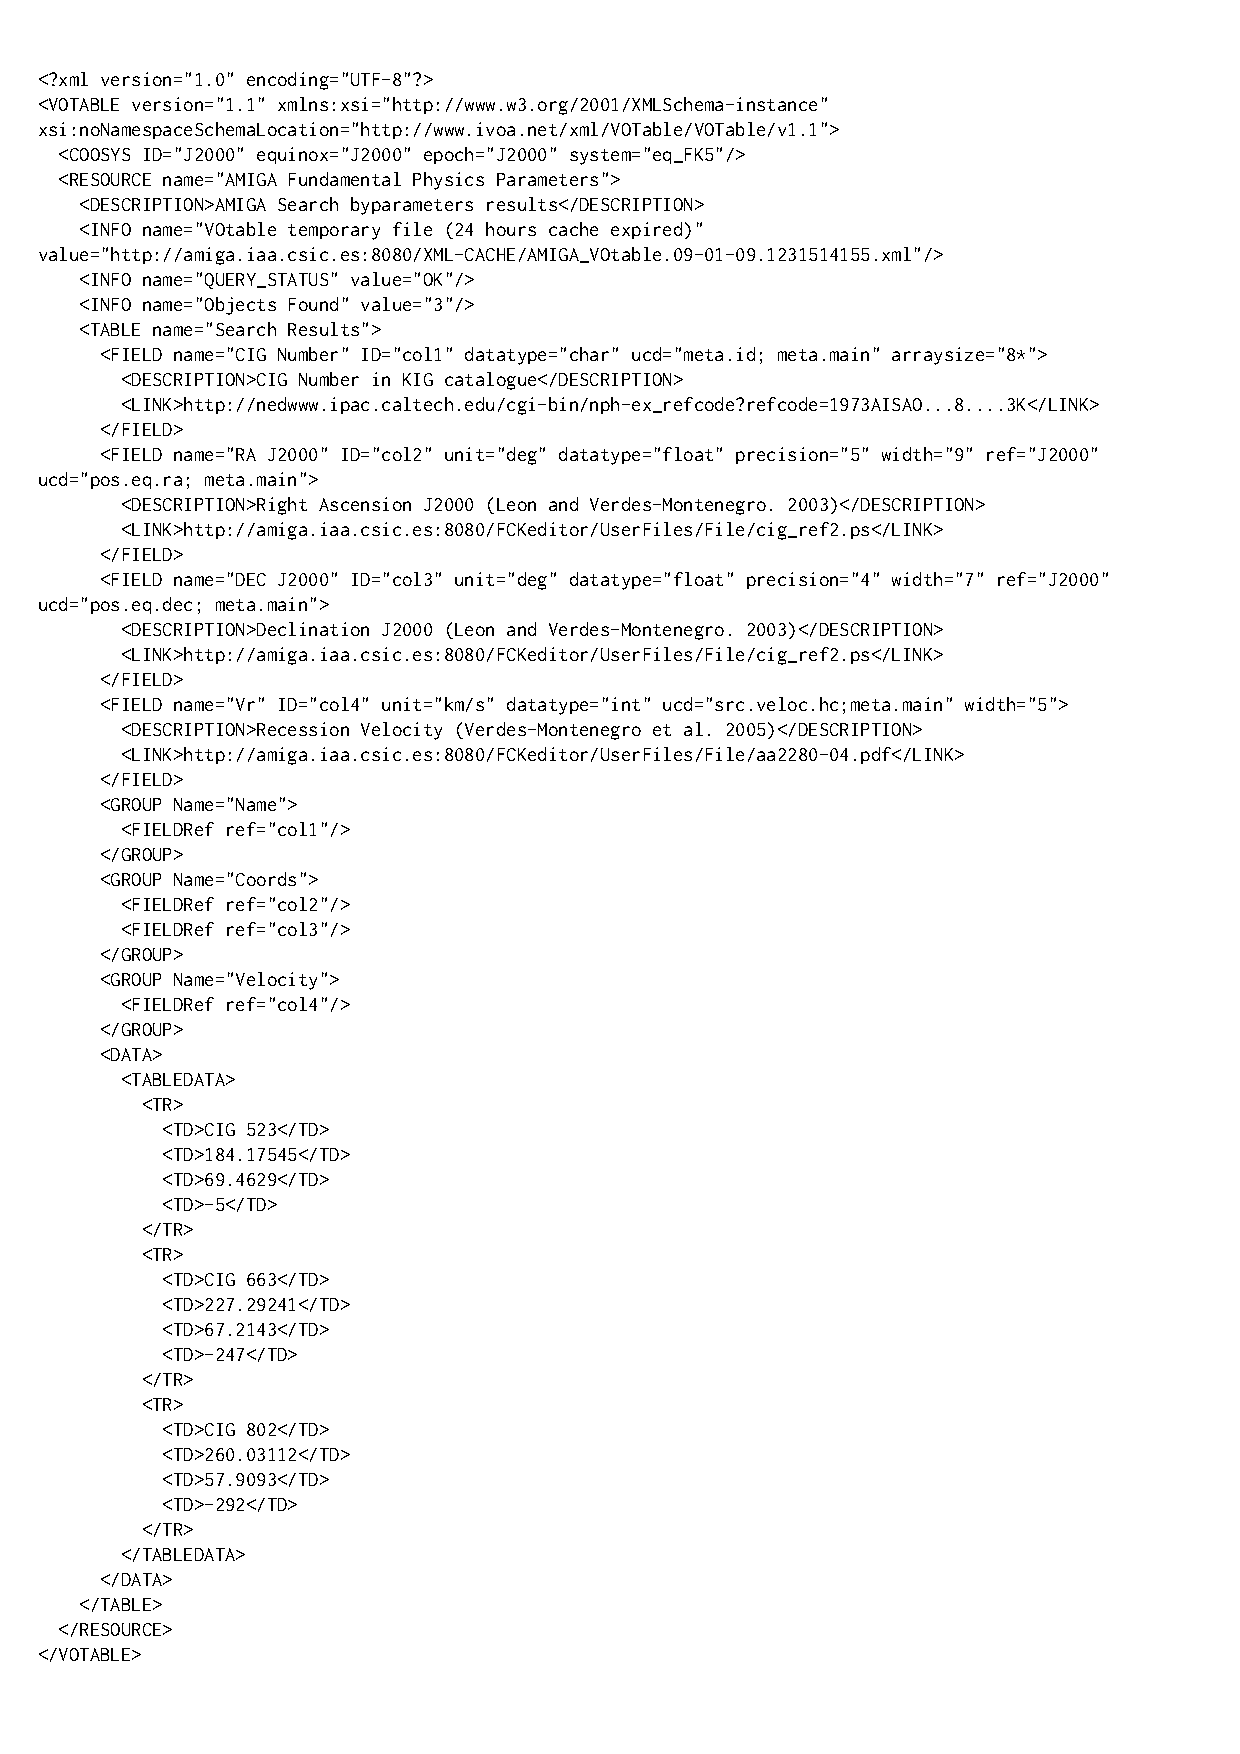
\includegraphics[height=0.787\textheight]
					{fig/amiga-vot.pdf}
				\caption[VOTable example]{
					Example of VOTable obtained from the AMIGA
					catalogue VO interface,
					\url{http://amiga.iaa.csic.es/DATABASE/}. We
					can see that after the initial XML declaration,
					and opening the \xmltag{VOTABLE}, the
					\xmltag{COOSYS} is used to specify the
					coordinate system equinox and epoch, and then
					the data is described in the
					\xmlopen{RESOURCE}/\xmltag{TABLE}. The
					\xmltag{FIELD} is used for every column in the
					table, the \xmltag{GROUP} is used to group
					together related fields, and then the
					\xmlopen{DATA}/\xmltag{TABLEDATA} contains the
					table rows between \xmltag{TR}s, and with
					columns separated by the \xmltag{TD}.
				}
				\label{fig:fig_amiga-vot}
			\end{figure}
					
			The complete definition of the VOTable, in terms of its
			XML Document Type Definition (DTD), and an XML Schema,
			can be found in
			appendix~\ref{cha:votable_format_definition}.
		
		% subsection the_votable (end)

%	The FITS file format intended to address two problems at the
%	time: standardising a data format for astronomical image and
%	tabular data interchange, and providing a computer
%	tape-friendly storage mechanism, with support for record
%	lengths multiple of common record lengths at the time.


%	, and in order to do that practically data had to be digitally
%	sampled. In fact, interferometry data conform a sparse sampling
%	of what is called the visibility plane, and imaging is made by
%	applying the Fourier Transform to that sparse sample. Models on
%	the originating data have to be imposed in order to do a proper
%	image reconstruction, and algorithms such as CLEAN, or Maximum
%	Entropy have been devised for that reconstruction.

	% section vo_data_formats (end)

	\section{VO data access protocols} % (fold)
	\label{sec:vo_data_access_protocols}
		
		The common file format helps in the data interchange
		between different systems, and in letting different
		applications share data. However, in order to retrieve
		those data from the different archives existing in the VO,
		common data access protocols are needed.
		
		 Then main astronomical data products produced as
		astronomical observation facilities are the reduced image,
		and the reduced 1D spectra. Working with those images and
		spectra, different properties of objects in the universe,
		such as temperature, distance, diameter, or more directly,
		received flux, Point Spread Function (PSF), et cetera, can
		be derived, and positional catalogues created.
		
		 For those kinds of data the initial VO protocols to be
		created were the Simple Image Access
		Protocol~\cite{2008sia..rprt.....T} (SIAP) and the Simple
		Spectral Access
		Protocol~\cite{Tody:2007yq,2004SPIE.5493..262D} (SSAP). For
		catalogues the Simple Cone Search (SCS, or ConeSearch)
		protocol~\cite{Williams:2008fv} was devised, with the idea
		of retrieving table rows from positional catalogues centred
		around a certain position, and from a certain angular
		distance from the centre (hence the Cone in the protocol
		name).
		
		 Apart from data-product driven access protocols, an
		additional data access protocol is needed for querying the
		VO Registry. That protocol is based on the Open Archives
		Initiative
		
		 You can find a brief description of each protocol
		interface in appendix~\ref{cha:vo_protocols} for quick
		reference.
		
	% section vo_data_access_protocols (end)

	\section{VO data models} % (fold)
	\label{sec:vo_data_models}
		
		With a common data format and a common data access protocol
		astronomers would be able to access different archives
		using automated tools, and the data could be sent to
		different applications.
		
		 However, astrophysical datasets are very complex in
		nature, and with the flexibility of the VOTable or the FITS
		file formats many different files can be constructed which
		contain the same astrophysical information, but in a
		incompatible form.
		
		 A data model is a description of the set of entities
		needed for information storage in a particular field, and
		specifies both the data being stored, and the relationships
		between them.
		
		 For the VO, there are several kinds of data models which
		can be built:
		
		\begin{description}
			\item[A general data model for astronomical
			observations] one such data model would be centred around
			the idea of astronomical observation and data reduction
			setup.
			
			 \item[Data model for individual data products] these
			data data models would exist for the different data
			products created with the different astronomical
			instruments: images, spectra, data cubes (collections
			of images or spectra), photometric data, et cetera.
		\end{description}
		
		In order to identify that a particular datum, appearing
		anywhere in a VO dataset, has a precise astronomical
		meaning the Unified Content Descriptors (UCDs) where
		created. They conform a controlled vocabulary whose precise
		meaning is set by the IVOA, and allow, for instance, to
		identify if a table column corresponds to flux in a
		particular radio band, or provides an astronomical
		coordinate, and so on.
		
		 We will see in Part~\ref{partRadioDataModelling} that the
		data modelling effort is still ongoing within the VO, and
		one of the main contributions of this thesis is a complete
		observation data model for radio astronomy, with some parts
		usable for non radio astronomical observations. More detail
		in UCDs will be offered there.

		%For instance, image mosaics can be delivered by a collection
		%of images in the same file with WCS information for each one;
		%or as a data cube with a different plane for each one of the
		%images, with a separate coordinates table related to each
		%plane; as a list of pixels with coordinates; as a series of
		%tables containing image data... the astronomical information
		%is the same, but we need to specify the kind of dataset
		%(astronomical image mosaic), and the relationship
		%
		%The VO needs, then, to be sufficiently structured so that
		%different applications and services provide the same metadata
		%for the same kind of data products, so that all applications
		%which know how to operate on certain datasets (images or
		%spectra, for instance, but also astronomical catalogues)
		%can find all the metadata they need for their operations.
		
		

		
		%There are two main kinds of astronomical data:
		%
		%\begin{description}
		%	\item[Data from observations] These are the most related
		%	to astronomical infrastructure. These are data coming from
		%	instruments in all kind of telescopes, and basically
		%	consist of the (more or less processed) output from light
		%	detectors.
		%	
		%	\item[Astronomical catalogues] Lists of astrophysical
		%	properties related to positions of the sky, which have been
		%	derived upon careful processing of observational data.
		%	These include purely physical parameters, such as
		%	temperatures, densities, masses, fluxes in different bands,
		%	et cetera; or attributes related with the observed object,
		%	such as object kind, morphology, names in pther catalogues,
		%	or even with the observational setup.
		%\end{description}
		%
		%%In astronomical observatories data is mainly in the form of
		%%observational data, but typically a catalogue of observed
		%%objects is generated.
		%%For surveys, the data is processed by an
		%%automatic processing pipeline which provides many different
		%%astronomical catalogues.
        %
		%As catalogue data is tabular in nature, the VOTable is a
		%perfect format for their distribution. However, they comprise
		%many diverse physical parameters, and it is very useful to
		%combine different catalogues to complement the physical
		%information. For instance, if we have infrared fluxes for an
		%object (from observations from an IR satellite, for instance),
		%but optical fluxes exist for the same object in a different
		%catalogue (from a ground based telescope, perhaps), combining
		%them will extend our knowledge of what is called the Spectral
		%Energy Distribution (SED)
		%of that object, and will helps in our
		%understanding of that object.
		%
		%In this case, we have three different problems to solve:
		%
		%\begin{enumerate}
		%	\item finding out catalogues which contain our object;
		%	
		%	\item cross-matching the catalogues, so that we can find
		%	out which objects in one catalogue correspond to the same
		%	object in other catalogue; this is implies being able to
		%	recognize in catalogues:
		%	
		%	\begin{itemize}
		%		\item which columns are devoted to astronomical 
		%		coordinates;
		%		\item find objects at a distance compatible with the
		%		precision of the astronomical coordinates
		%		(cross-matching);
		%	\end{itemize}
		%	
		%	\item identify exactly which properties are found in each
		%	column.
		%\end{enumerate}
		

		

		
	%	\todo{Revise the idea of semantics}
	%	We have talked several times about how VOTables, the common
	%	IVOA data format, allows data providers to specify data models
	%	and semantics for particular columns.
    %
	%	We understand semantics as the set of metadata which is used
	%	to allow automatic discovery of data roles. Part of that
	%	semantics come from the particular field where the data is
	%	being generated or applied, and are coded into the particular
	%	data model applied to the field.
    %
	%	In the VO, there are three kinds of attributes devoted to
	%	provide semantics to tagged data in VOTables: units, UCDs, and
	%	UTypes.
    %
	%	\subsection{Units} % (fold)
	%	\label{sub:units}
    %
	%	Mathematical operations on physical quantities can only be
	%	consistently performed on unit-compatible fields. For a
	%	tabular data and astrophysical image transport mechanism,
	%	be it FITS or VOTable, specifying the units for the
	%	different fields or pieces of data is almost mandatory.
	%	Even when the FITS standard does not mandate units to be
	%	provided, it recommends their use. In the same spirit, the
	%	unit attribute for VOTable tags is not mandatory, but it is
	%	strongly recommended.
    %   
	%	There is also a provision for constructing dimensional
	%	equations and other string units, but several equivalent
	%	ways of specifying those equations are allowed, instead of
	%	establishing an unambiguous construction rule.
    %   
	%	Within the Virtual Observatory, the Semantics Working
	%	Group has a dedicated group to Units.
	%	\textbf{Pedro Osuna and Jesús Salgado}
	%	made a concrete proposal for uniquely specifying
	%	both units and dimensional equations in the context of
	%	astrophysical spectra~\cite{2005astro.ph.11616O}.
    %   
	%	In particular, they proposal makes use of the Dimensional
	%	Analysis in order to show that, more than simple units, the
	%	dimensional equation, and scaling factors with respect to
	%	SI (System Internationale) units,
	% are enough to allow automatic comparison and
	%	re-scaling and interoperation between spectra with either
	%	frequency or wavelength units, 
	%	and flux densities with respect to
	%	frequency or wavelength (a non trivial task). Additional
	%	\texttt{dimeq} and \texttt{scaleq} attributes for specifying
	%   unit scales and dimensional equations in a
	%	VOTable, or \texttt{CSCALEQ} and \texttt{CDIMEQ} FITS
	%	keywords have to be added for each axis to provide unit
	%	interoperation.
    %   
	%	They have already implemented their recommendation in
	%	their VOSpec spectral analysis and SED synthesis tool, in
	%	order to be able to assemble spectral energy distributions
	%	from spectra in the whole emission range, from radio to
	%	X-rays. In that sense, errors must also be provided, with
	%	their corresponding units.
    %   
	%	Dimensional analysis is key for unit semantics in the
	%   Virtual Observatory data. With access to
	%	dimensional equations, automatic data mining of properties
	%	of large samples can derive a reliable functional fit of
	%	the dependency between observable quantities, by obtaining
	%	the independent adimensional products of observable
	%	parameters, and testing different functional forms of those
	%	adimensional products for the best fit to observational
	%	data~\cite{2007arXiv0709.3584T}.
    %
	%	% subsection units (end)
    %
	%	\subsection{Unified Content Descriptors (UCDs)} % (fold)
	%	\label{sub:unified_content_descriptors}
	%		
	%	Specifying both units and the unit reference base (usually,
	%	the SI, but many times, and for specific areas of
	%	astrophysics such as cosmology or high energy astrophysics,
	%	other unit base systems are adopted) is mandatory to allow
	%	commensurable data to be compared.
	%	
	%	However, many times quantities of the same nature, but
	%	different origin, coexist in the same table. For instance,
	%	one might have a table of flux measured at several
	%	wavelengths. All columns will share the same flux units
	%	(or, in any case, they can be automatically converted by
	%	means of dimensional attributes), but have a different
	%	meaning for an astrophysicist. Distinguishing between
	%	unit-compatible fields with different astrophysical meaning
	%	is the role of the UCDs~\cite{2004ASPC..314..315D}.
	%	
	%	UCDs were developed for the
	%	VizieR\urlnote{http://vizier.u-strasbg.fr/} online
	%	astronomical catalogue storage and query
	%	system~\cite{2000A&AS..143...23O} in the context of the
	%	ESO/CDS data mining project~\cite{1999ASPC..172..379O}, in
	%	order to harmonise the labelling (semantics) of similar
	%	fields between catalogues submitted from different research
	%	groups across the world\footnote{A classical example is the
	%	labelling of magnitudes in the V filter of the Johnson
	%	photometric system. Prior to the introduction of UCDs,
	%	there were up to 150 different labels for columns including
	%	information of that magnitude.}. Only if truly equivalent
	%	columns are compared can knowledge be reliably extracted.
	%	By using a controlled vocabulary, it is possible to find
	%	comparable information from different sources (for
	%	performing statistics on large samples, for instance).
	%	
	%	Still, even when UCDs are truly useful when comparing
	%	catalogues, and are very
	%	\textbf{interesting} for the discovery of
	%	what information might be comparable, they are not enough
	%	for specifying the role of a given datum in a larger
	%	context. For that, we need data models, and a way to
	%	specify relationships of a single datum with data model
	%	entities and attributes.
	%		
	%	% subsection unified_content_descriptors (end)
    %
	%   \subsection{Data models in the VO} % (fold)
	%   \label{sub:data_models_in_the_vo}
    %
	%   \todo{
	%   	\begin{itemize}
	%   		\item Existing VO data models
    %
	%   		\begin{itemize}
	%   			\item Characterisation
    %
	%   			\item Spectrum/Spectral Energy Distribution
	%   		\end{itemize}
    %
	%   		\item Missing VO Data Model classes
    %
	%   		\begin{itemize}
	%   			\item Provenance
	%   			\item Policy
	%   			\item Packaging
	%   			\item Target
	%   			\item Observation
	%   		\end{itemize}
    %
	%   		\item New VO Data models in this thesis
    %
	%   		\begin{itemize}
	%   			\item Provenance
	%   			\item Policy
	%   			\item Packaging
	%   		\end{itemize}
    %
	%   		\item RADAMS
	%   	\end{itemize}
	%   }
			
			
			
		% subsection data_models_in_the_vo (end)


	% section sec:vo_data_models (end)

	\section{VO applications} % (fold)
	\label{sec:vo_applications}

		VO data formats, access protocols, and data models are the
		infrastructure on which the rest of the VO relies. We
		call \emph{VO application} to any software package of any
		kind which makes use of existing VO services to perform
		the visualisation of data in VO format, queries of VO
		services, or even computations on existing datasets either
		in VO format, or retrieved from the VO.
		
		 However, having VO users in mind, it is best to classify
		applications depending on whether they allow users and/or
		developers to create new packages, or if they are intended
		to be used for scientific analysis. And in this latter
		case, the kind of scientific use they support.
		
		 We have provided a series of tables with a non-exhaustive
		list of different classes of VO applications:
		table~\ref{tabVODataDiscoveryApps} compiles VO applications
		for data discovery; table~\ref{tabVODataHandlingApps}
		combines applications for data manipulation and handling;
		VO applications specific for spectral analysis are shown in
		table~\ref{tabVOSpectralApps}; table~\ref{tabVODevelTools}
		shows tools, libraries, and reference portals to the VO for
		application developers; finally, difficult to classify VO
		resources can be found in table~\ref{tabVOotherApps}.
		
	 	%%todo (fold)
		%\todo{
		%	For each of these....
		%	\begin{itemize}
		%		\item Registry queries
		%		\item ConeSearch queries
		%		\item SIAP queries
		%		\item SSAP queries
		%	\end{itemize}
	    %
		%	Specify:
		%	\begin{itemize}
		%		\item Application name
		%		\item URL
		%		\item Strengths
		%		\item Weaknesses
		%	\end{itemize}
		%}
		%%todo (end)

			\newcommand{\ivoaappsurl}
	{\concatenate{http://www.ivoa.net/cgi-bin/}
	{twiki/bin/view/IVOA/IvoaApplications}}
	\newcommand{\fromlist}
	{
		from the \href{\ivoaappsurl}{IVOA},
		\href{http://www.us-vo.org/projects/tools.cfm}{NVO} and
		\href{http://www.euro-vo.org/pub/tc/software.html}{EuroVO
		TC} applications and tools' lists.
	}
	
	\begin{table}
	\begin{center}
	\begin{scriptsizetabular}{p{2.8cm}p{9.5cm}}
	
	\textbf{Application} &
	% \textbf{Contact Person} &
	\textbf{Description} \\ \midrule
	
	\href{http://aladin.u-strasbg.fr/} {Aladin} & Interactive
	federated sky atlas.\\ \addlinespace
	
	\href{http://heasarc.gsfc.nasa.gov/vo} {NVO Datascope} & 
	Portal for positional queries to all NVO registered services.
	\\ \addlinespace
	
	\href{http://www.cadc-ccda.hia-iha.nrc-cnrc.gc.ca/cvoProto/}
	{Octet} & CVO Registry Observation CaTalog Exploration Tool.
	% Queries the CVO registry, provides data cross-matching.
	\\ \addlinespace
	
	\href{http://www.astrogrid.org/wiki/Help/IntroVODesktop}
	{VODesktop} & A resource-centered desktop client for VO:
	includes VOExplorer, Query and Task Runner, Astroscope, VOSpace
	Browser, Astro Runtime. \\ \addlinespace
	
	\end{scriptsizetabular}
	\end{center}
	\caption[List of VO data discovery applications]
	{List of VO data discovery tools and applications, \fromlist}
	\label{tabVODataDiscoveryApps}
	\end{table}
	
	
	\begin{table}
	\begin{center}
	\begin{scriptsizetabular}{p{2.8cm}p{9.5cm}}
	
	\textbf{Application} &
	% \textbf{Contact Person} &
	\textbf{Description} \\ \midrule
	
	\href{http://www.cacr.caltech.edu/projects/nvo/atlasmaker/3}
	{Atlasmaker} & Grid software for bulk image resampling.\\
	\addlinespace
	
	\href{http://cm.bell-labs.com/who/tkh/mirage/index.html}
	{Mirage} & Multi-dimensional visualisation of data from VOTable
	source files.\\ \addlinespace
	
	\href{http://montage.ipac.caltech.edu/} {Montage} &
	Science-grade custom mosaics from a portal.\\ \addlinespace
	
	\href{http://iraf.noao.edu/projects/vo/votool/} {NOAO VOTool} &
	A visual VOTable authoring and editing tool. \\
	\addlinespace
	
	\href{http://iraf-nvo.noao.edu/wcsfixer/} {NOAO WCSFixer} &
	Automatic WCS correction for uploaded images. \\ \addlinespace
	
	\href{http://www.atnf.csiro.au/vo/rvs} {Remote Visualisation
	System (RVS)} & Distributed software for visualisation and
	analysis of remotely located astronomical images with VO
	support. \\ \addlinespace
	
	\href{http://www.star.bristol.ac.uk/~mbt/topcat/} {TOPCAT} &
	Viewer and editor for tabular information. Based on the
	STILTS tool set.\\ \addlinespace
	
	\href{http://www.starlink.ac.uk/treeview/} {Treeview} &
	Hierarchical data format viewer with XML and
	VOTable support. \\ \addlinespace
	
	\href{http://visivo.cineca.it/} {VisIVO} & A VO-compatible
	visualisation tool for large datasets. \\ \addlinespace
	
	\href{http://vo.iucaa.ernet.in/~voi/voplot.htm} {VOPlot} &
	Tool for visualizing astronomical data from VOTable sources.\\
	\addlinespace
	
	\href{http://services.china-vo.org/vofilter/} {VOFilter} & XML
	filter for OpenOffice Calc to Read/Write VOTable Files.\\
	\addlinespace
	
	\href{http://services.china-vo.org/votable2xhtml/}
	{VOTable2XHTML} & XSLT Style-sheet for exporting VOTable files
	to HTML.  \\
	\addlinespace
	
	\href{http://nvogre.phyast.pitt.edu:8080/wesix/} {WESIX} &
	\emph{Web Enabled Source Identification with X-matching},
	portal for image upload, source extraction, and cross
	correlation with selected survey catalogues.
	
	\end{scriptsizetabular}
	\end{center}
	\caption[List of VO data handling and manipulation
	applications]
	{List of VO data handling and manipulation applications,
	\fromlist}
	\label{tabVODataHandlingApps}
	\end{table}
	
	
	
	\begin{table}
	\begin{center}
	\begin{scriptsizetabular}{p{2.8cm}p{9.5cm}}
	
	\textbf{Application} &
	% \textbf{Contact Person} &
	\textbf{Description} \\ \midrule
	
	\href{http://voplus.obspm.fr/~chil/Euro3D/}
	{Euro3D} & Spectral analysis tool for Euro3D formatted
	Integral Field Units (IFUs) datasets, by Igor
	Chilingarian.\\
	\addlinespace
	
   \href{http://www.stsci.edu/resources/software_hardware/specview}
	{Specview} & Visualisation and analysis tool for 1-D
	astronomical spectrograms.\\ \addlinespace
	
	\href{http://star-www.dur.ac.uk/~pdraper/splat/splat-vo/}
	{SPLAT} & Spectral Analysis Tool from Starlink. \\
	\addlinespace
	
	\href{http://svo.laeff.inta.es/theory/vosa2//}{VOSA} &
	A web-based tool developed by the SVO for automatic
	analysis of
	Spectral Energy distributions from online spectra.\\
	\addlinespace
	
	\href{http://sdc.laeff.inta.es/vosed/}{VOSED} & A web-based
	tool
	developed by the SVO for
	building Spectral Energy distributions from online spectra.\\ 
	\addlinespace
	
	\href{http://www.star.bris.ac.uk/~mbt/yafit/}{Yafit} & Yet
	Another Fitting tool for fitting curves to data points,
	which can be used to fit model spectra to observed photo
	metric data points, by Mark Taylor.\\ 
	\addlinespace
	
	\newcommand{\sciopsbaseurl}[0]
	{http://www.sciops.esa.int/index.php}
	\href{\sciopsbaseurl?project=ESAVO}{VOSpec} &
	A Tool to Handle VO-SSAP compliant spectra.\\ \addlinespace
	
	\end{scriptsizetabular}
	\end{center}
	\caption[List of VO spectral analysis and SED fitting
	applications]
	{List of VO applications for spectral analysis and
	spectral energy distribution (SED) fitting, \fromlist}
	\label{tabVOSpectralApps}
	\end{table}
	
	
	
	
	\begin{table}
	\begin{center}
	\begin{scriptsizetabular}{p{2.8cm}p{9.5cm}}
	\textbf{Developer Tool} &
	% \textbf{Contact Person} &
	\textbf{Description} \\ \midrule
	
	\newcommand{\arpythonurl}[0]
	{\concatenate{http://deployer.astrogrid.org/software/}
	{astro-runtime/commandline/index.html}}
	\href{\arpythonurl}
	{AR Command line} & Python wrapper for the AstroRuntime
	VO middleware. \\ \addlinespace
	
	\href{http://cdsweb.u-strasbg.fr/cdsdevcorner/} {CDS Developer's
	Corner} & Web site for developers of the Centre de Donées de
	Strasbourg, where references to CDS web-services and CDS Java
	software can be found, including unit handling. \\
	\addlinespace
	
	\href{\jsampurl}
	{JSAMP} &
	JSAMP is a Java implementation of the SAMP messaging
	protocol written in Java by Mark Taylor.\\
	\addlinespace
	
	\href{\caltechphpurl}{PHP VO Client Library} & 
	PHP interface classes to ConeSearch, SIAP, SkyNode,
	and VORegistry services.\\
	\addlinespace
	
	\href{\caltechpythonurl}{Python VO Client Library} &
	Python interface classes to ConeSearch, SIAP, SkyNode,
	and VORegistry services.\\
	\addlinespace
	
	\href{http://amwdb.u-strasbg.fr/saada} {Saada} &
	Auto-configurable database generator and VO Service publisher
	for medium to small sized datasets, directly from FITS files.
	\\ \addlinespace
	
	\href{\sampyurl}
	{SAMPy} & SAMPy is a Python implementation of the SAMP
	messaging protocol, with additions to allow for SAMPy
	applications to communicate with remote computer, and not just
	locally. By Luigi Paioro.\\
	\addlinespace
	
	\href{http://cdsweb.u-strasbg.fr/cdsdevcorner/savot.html}
	{SAVOT} &
	Simple Access to VOTable, SAVOT is a Java-based library to
	parse VOTable documents, written by André Schaaff from the
	CDS.\\
	\addlinespace
	
	\href{\stiltsurl} {STILTS} &
	Command-line tools for arbitrarily large table manipulation
	and format conversion, including FITS and VOTable formats.
	By Mark Taylor.\\
	\addlinespace
	
	\href{http://iraf-nvo.noao.edu/vo-cli/} {VO-CLI} &
	Command-line Tools for the VO, to be used with IRAF. \\
	\addlinespace
	
	\end{scriptsizetabular}
	\end{center}
	\caption[List of VO development resources]
	{List of VO developer utilities, libraries, and resources,
	\fromlist}
	\label{tabVODevelTools}
	\end{table}
	
	\begin{table}
	\begin{center}
	\begin{scriptsizetabular}{p{2.8cm}p{9.5cm}}
	
	\textbf{Application} &
	% \textbf{Contact Person} &
	\textbf{Description} \\ \midrule
	
	\href{http://bima.astro.umd.edu/nemo/tvo/nvodemo2004/} {GC
	Theoretical Models} & Prototype tool for comparing
	globular cluster (GC) simulations with observed
	color-magnitude diagrams.\\ \addlinespace
	
	\href{http://www.nvo.noao.edu} {NOAO NVO Portal} &
	VO portal providing different views for NOAO-hosted data.
	%Provides a unified UI for different archives, including
	%calendar and footprint views.
	\\ \addlinespace
	
	\href{http://pegasus.isi.edu/} {Pegasus} & Workflow Management
	on the Grid.\\ \addlinespace
	
	\href{http://hea-www.harvard.edu/~arots/nvometa/} {STC
	Metadata} & Space-Time Coordinate metadata for the VO.\\
	\addlinespace
	
	\href{http://voservices.org/} {VO Services} & A growing
	selection of VO services in production.\\ \addlinespace
	
	\href{http://nvogre.phyast.pitt.edu:8080/wesix/} {WESIX} &
	\emph{Web Enabled Source Identification with X-matching},
	portal for image upload, source extraction, and cross
	correlation with selected survey catalogs.
	
	\end{scriptsizetabular}
	\end{center}
	\caption[List of other VO applications and portals]
	{Other VO applications and portals not presented yet, \fromlist}
	\label{tabVOotherApps}
	\end{table}
	

	% section vo_applications (end)

	\section{VO inter-application messaging} % (fold)
	\label{sec:vo_application_messaging}
	
		The data access protocols mentioned in
		section~\ref{sec:vo_data_access_protocols} need the
		deployment of a full-featured web server. However, in a
		local machine, with several VO applications running at the
		same time, and with all of them understanding VOTables and
		FITS files, a simple messaging protocol between
		applications would allow them to notify, or be notified,
		that some data is available, and if the messaging protocol
		supported it, several applications in communication could
		be showing different but interacting views of the same
		data.
		
		 Such a messaging protocol was prototyped and was initially
		known as the PLatform for Astronomical Tool InterConnection
		(PLASTIC), and implemented in many different VO
		applications, such as TOPCAT, or the Aladin Sky Atlas. The
		shortcomings of the PLASTIC protocol gave birth to the
		Simple Application Messaging Protocol (SAMP), now in
		Proposed Recommendation stage.
		
		 The SAMP messaging protocol is described in
		section~\ref{sec:samp_messaging}.
	
	% section vo_application_messaging (end)
	
	\section{VO resource registry} % (fold)
	\label{sec:vo_resource_registry}
	
		The only way VO clients can remain aware of existing and
		newly incorporated services is by means of a registration
		point were public data services are announced.
		
		 In the VO, there is no centralised, preferential registry.
		Instead, many registries exist, but with the ability to
		harvest entries from other registries, so that there can
		exist specialised registries on one hand, and shared
		registries entries on the other.
		
		 VO registry and harvesting infrastructure has been built
		around the Open Archives
		Initiative\urlnote{http://www.openarchives.org/} (OAI)
		standard resource registries, so that an already in place
		infrastructure could be leveraged. The OAI has developed a
		Protocol for Metadata Harvesting
		(OAI-PMH)~\cite{2002OAI-PMH}, that allows OAI registries to
		harvest other OAI registries they might know about (with an
		entry in their own registry, for instance), so that VO
		resources can be entered in one registry, and they should
		propagate to any other OAI-PMH compliant registries.
		
		 That allows VO tools to point to a single harvesting
		registry, and rest assured that VO servers will be found in
		any of those registries.
		
		 Registered resources (OAI-PHM records) provide at least
		the Dublin Core metadata set~\cite{2007NISO.Z3985...K},
		which specifies resource types, publishers, curators, et
		cetera.
		%See table~\ref{tab:DublinCoreMetadata}
		%for the complete list of Dublin Core keywords.
		Additionally, service-specific resource profiles exist for
		the different data access service types, and include
		astronomical data for service such as the sky region
		covered by the observation ---footprint---, wavelength,
		instruments providing the data, et cetera.
		
		 In particular, the VOResource~\cite{2008voresivoar0222P}
		XML Schema has been developed as the acceptable OAI-PHM
		record formats for generic VO registries, and the
		VODataService schema~\cite{2008vods.ivoar1016P} is in
		development to further standardise data service entries.
		
		 Several VO registries provide web pages to query the
		registries apart from the usual OAI-PHM interface, such as
		the NVO
		Carnivore\urlnote{http://nvo.caltech.edu:8080/carnivore/},
		or the ESA-VO
		registry\urlnote{http://esavo.esa.int/registry/}.
	
	% section vo_resource_registry (end)
	
	% section the_international_virtual_observatory_alliance (fold)
	\section[The International Virtual Observatory Alliance]
	{Standardising the VO:
	 the International Virtual Observatory Alliance (IVOA)}
	\label{sec:the_international_virtual_observatory_alliance}

		% \lourdes{Buscar sitio para párrafo intro IVOA.}
		As previously stated, for VO common data formats,
		interfaces, and data models to become truly standard
		requires a standards enforcing authority, and within the VO
		the International Virtual Observatory Alliance (IVOA) is
		the organisation in charge of developing and sanctioning
		interoperability standards.
		
		 The International Virtual Observatory Alliance was created
		in 2002, after the first national VO associations realised
		that they needed to keep working together, and that an
		international standards-setting organisation was needed to
		sanction Virtual Observatory standards, steer the
		development of new ones, and foster the spread of the VO to
		most data providers.
		
		 The IVOA founders were the US National Virtual Observatory
		(NVO), the European (AVO) and supporting centres ---Centre
		de Données astronomiques de Strasbourg (CDS), AstroGrid,
		German Astrophysical Virtual Observatory (GAVO)---, the
		Russian Virtual Observatory (RVO), VO-India, e-Astronomy
		Australia (eAA; later Australian Virtual Observatory,
		Aus-VO) and the Canadian Virtual Observatory (CVO), which
		in 2002 met at the ESO Headquarters in Garching, and agreed
		in forming the International Virtual Observatory Alliance,
		following the statement drafted by Peter Quinn, Robert
		Hanisch, and Andy Lawrence~\cite{Quinn:2002qf}. The minutes
		of that meeting can be found in~\cite{deYoung:2002rt},
		and the conference proceedings compiled in the book
		\emph{Toward an International Virtual
		Observatory}~\cite{2004tivo.conf.....Q}.
		
		 Following that initial meeting, several services were
		created, and Aladin was provided with a VO interface,
		giving birth to the first Astrophysical Virtual Observatory
		(AVO) prototype~\cite{2004ASPC..314..304Q}.
		
		 The inspiration for the IVOA organisation is the World
		Wide Web Consortium\urlnote{http://w3c.org/} (W3C), in the
		sense of providing the steering effort for standards to be
		agreed upon within different Working Groups (WGs), so that
		there is an official forum in which such standards are
		proposed, discussed, and finally approved. The main
		difference with the W3C is that the latter is \emph{pay per
		play} ---W3C participants pay in order to influence the
		standardisation process---, while the IVOA is open to any
		interested party with expertise in a given field.
		
		Presently \invisiblenote{(as of August 2008)}, the IVOA is
		formed by 16 VO projects from all over the
		world\urlnote{http://ivoa.net/pub/members/}, from Armenia,
		Australia, Canada, China, Europe, France, Germany, Hungary,
		India, Italy, Japan, Korea, Russia, Spain, the United Kingdom,
		and the United States (see figure~\ref{fig:fig_IVOAMembers}).
		Membership is open to additional national and international
		projects\footnote{
			VO projects wishing to join the IVOA must
			follow the IVOA Guidelines for Participation
		\url{http://ivoa.net/Documents/latest/IVOAParticipation.html}.
		}.

		\begin{figure}[tbp]
			\centering
				
\includegraphics[width=\columnwidth]
				{fig/ivoa-members.png}
			\caption[IVOA member organisations]
			{
				The 16 IVOA member organisations, as of August
				2008. The Spanish Virtual Observatory (SVO) joined
				the IVOA in 2004. Several European countries have
				their own national VO initiatives (France's
				VO-France, Germany's GAVO, Italy's VObs.it, Spain's
				SVO, UK's AstroGrid), which also form part of the
				European Community funded Euro-VO.
			}
			\label{fig:fig_IVOAMembers}
		\end{figure}

		\newcommand{\svourl}[0]{http://svo.laeff.inta.es/}
		
		 The Spanish participation in IVOA is performed through the
		Spanish Virtual Observatory\urlnote{\svourl}
		(SVO)~\cite{2006ASPC..351...19G}. The seed for the SVO
		were the efforts of the Laboratorio de Astrofísica Espacial
		y Física Fundamental (Laboratory for Spatial Astrophysics
		and Fundamental Physics, LAEFF\footnote{LAEFF is part of
		the National Institute for Aerospatial Technologies, INTA})
		to build a VO-compliant archive from the IUE Newly
		Extracted Spectra (INES) archive\footnote{In fact, the VO
		INES archive was one of the first spectroscopic archives to
		be available to the VO.}.
		% Nowadays the main FTEs are provided by the
		% LAEFF-INTA (SVO-core), but additional FTEs are provided by
		% other partners, such as the IAA-CSIC, and there is a national
		% network which funds the participation of additional research
		% groups within the Virtual Observatory.
		This thesis is part of the IAA contribution to the SVO.
		
		 As mentioned earlier, the IVOA is a standards-sanctioning
		organisation and a steering force for the development of
		interoperability protocols, applications, and best
		practices regarding the Virtual Observatory. As seen on
		previous sections, there are different development areas
		within the VO, and there exist several Working Groups
		focused in each particular area. There are also Interest
		Groups which do not focus in actual development, but
		instead serve as a discussion forum for issues not directly
		pertaining to the Virtual Observatory, but which might
		eventually end up forming part of it.

		 The main IVOA organisational building blocks are Working
		Groups, Interest Groups, and Coordination and steering
		committees. Their detailed discussion can be found in
		Appendix~\ref{cha:the_ivoa}.
		Figure~\ref{OrganisationalBuildingBlocksIVOA} shows
		graphically the high-level organisation of the IVOA.
		
		\begin{figure}[tbp]
			\centering
				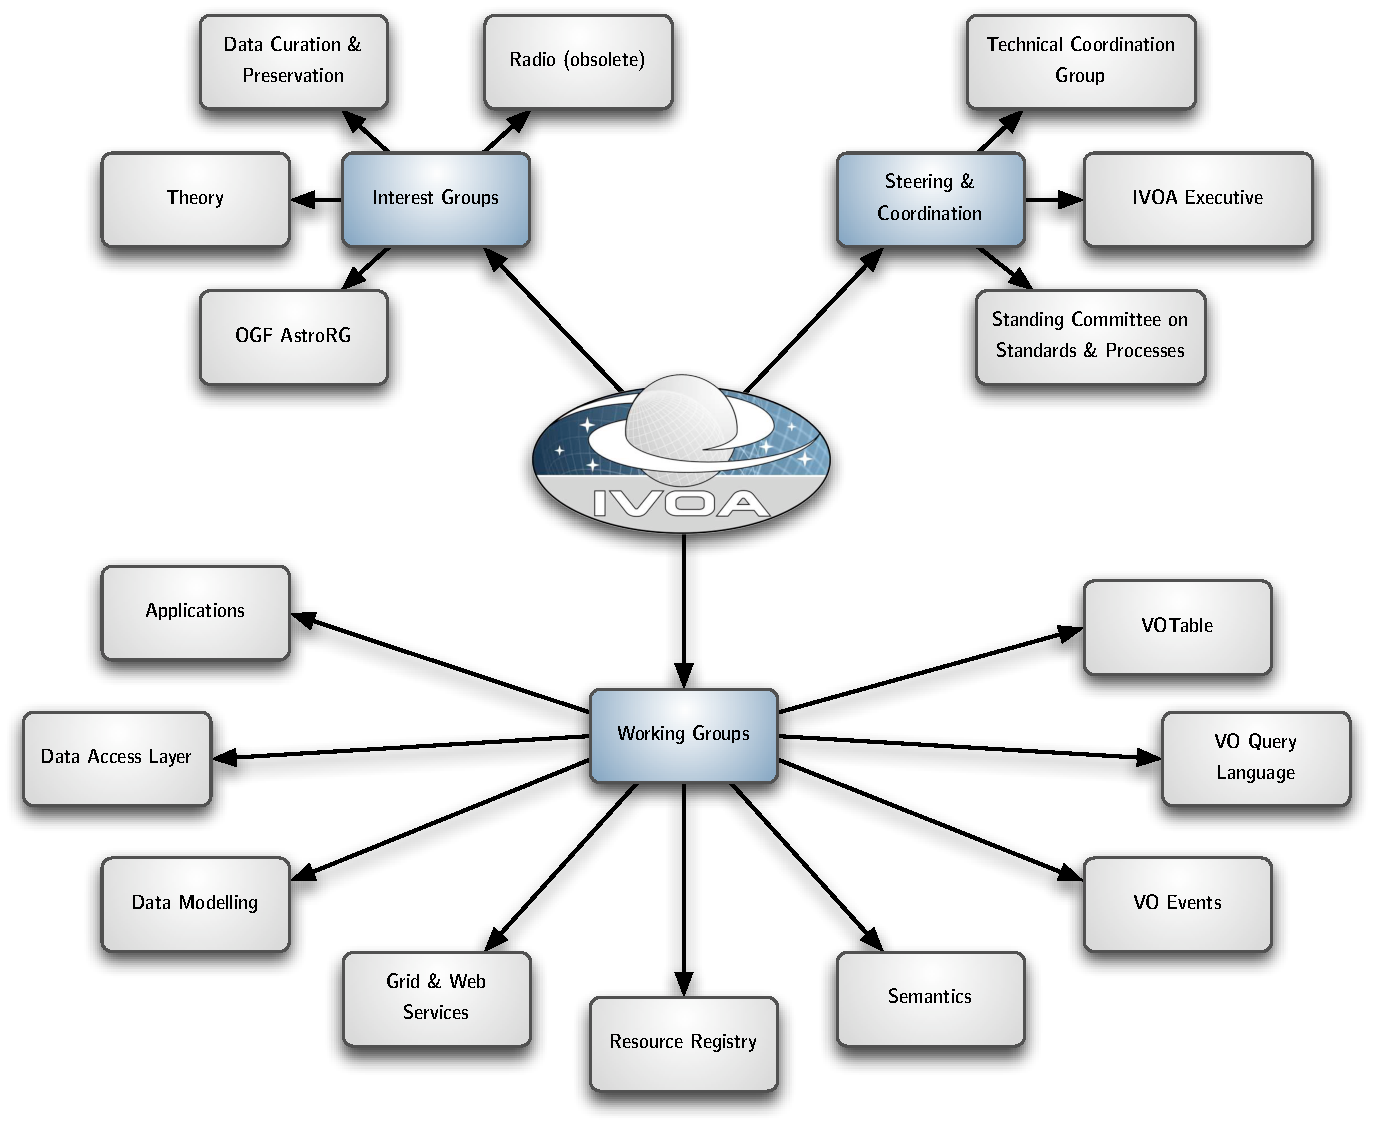
\includegraphics[width=\columnwidth]
				{fig/OrganisationalBuildingBlocksIVOA.pdf}
			\caption[IVOA organisational building blocks]{
				IVOA organisational building blocks: Working
				Groups, Interest Groups, and Coordination boards.
				The IVOA activity for standards development is
				performed in the Working Groups, while Interest
				Groups gather together IVOA users with common
				interests outside the Virtual Observatory (such as
				the Open Grid Forum, or the Data Curation and
				Preservation interest groups), or outside existing
				Working Groups (such as the Radio astronomy or or
				Theory interest groups). The Steering \&
				Coordination bodies provide the main direction for
				IVOA activities, technical coordination across the
				existing Working Groups (i.e., Data Modelling and
				Data Access Layer in the development of
				interoperable protocols and data set access tools),
				and take care of possible changes to existing
				standards.
			}
			\label{OrganisationalBuildingBlocksIVOA}
		\end{figure}
		
		IVOA Working Groups are not completely equal in scope. Most
		of them have to do with particular parts of the IVOA, as
		seen in figures~\ref{fig:fig_VOArch} and
		\ref{fig:fig_VOAPIStack}.
		
	% section the_international_virtual_observatory_alliance (end)


\section{The VO from the point of view of different actors} % (fold)
\label{sec:the_vo_from_the_point_of_view_of_different_actors}

	Which parts of the Virtual Observatory do users interact with?
	What does a particular astronomer need to know?
	
	 In the following subsections we will offer several portraits
	of the VO as seen from the points of view of different actors:
	the astronomical user, the application developer, the data
	provider, and the data service developer.

	\subsection{The VO from the user's point of view} % (fold)
	\label{ssub:the_vo_from_the_point_of_view_of_the_user}
	
	
		\newcommand{\specviewurl}[0]
		{http://www.stsci.edu/resources/software_hardware/specview}
		\newcommand{\splatvourl}[0]
		{http://astro.dur.ac.uk/~pdraper/splat/splat-vo/}
		\newcommand{\vodesktopurl}[0]
		{http://www.astrogrid.org/wiki/Install/Downloads}
	
		For a non-technical user (one who wishes to use the VO via
		standard tools, and does not wish to access directly the VO
		infrastructure), the VO can be seen just as a set of
		portals (applications or web sites) which access all of the
		services and data available in the Virtual Observatory.
		Some of them might also retrieve additional data from
		non-VO-compliant archives, and even mix them with local
		datasets. Users would launch different VO applications
		depending of the tasks they might wish to perform (Aladin
		Sky Atlas\urlnote{http://aladin.u-strasbg.fr/} for
		catalogue and image queries;
		TOPCAT\urlnote{http://www.star.bris.ac.uk/~mbt/topcat/} for
		catalogue and table manipulation;
		VOSpec\urlnote{http://esavo.esa.int/vospec/},
		SpecView\urlnote{\specviewurl} or
		SPLAT-VO\urlnote{\vodesktopurl} for spectra manipulation;
		VODesktop\urlnote{\vodesktopurl} for Registry queries,
		remote task execution, and access to the VOSpace; or web
		portals such as the NVO
		Datascope\urlnote{http://heasarc.gsfc.nasa.gov/vo/} for
		all-encompassing browser-based archive searches). See
		figure~\ref{fig:figUserPOV_VOArch} for a conceptual diagram
		of the VO for astronomers.
		
		\begin{figure}[btp]
			\centering
				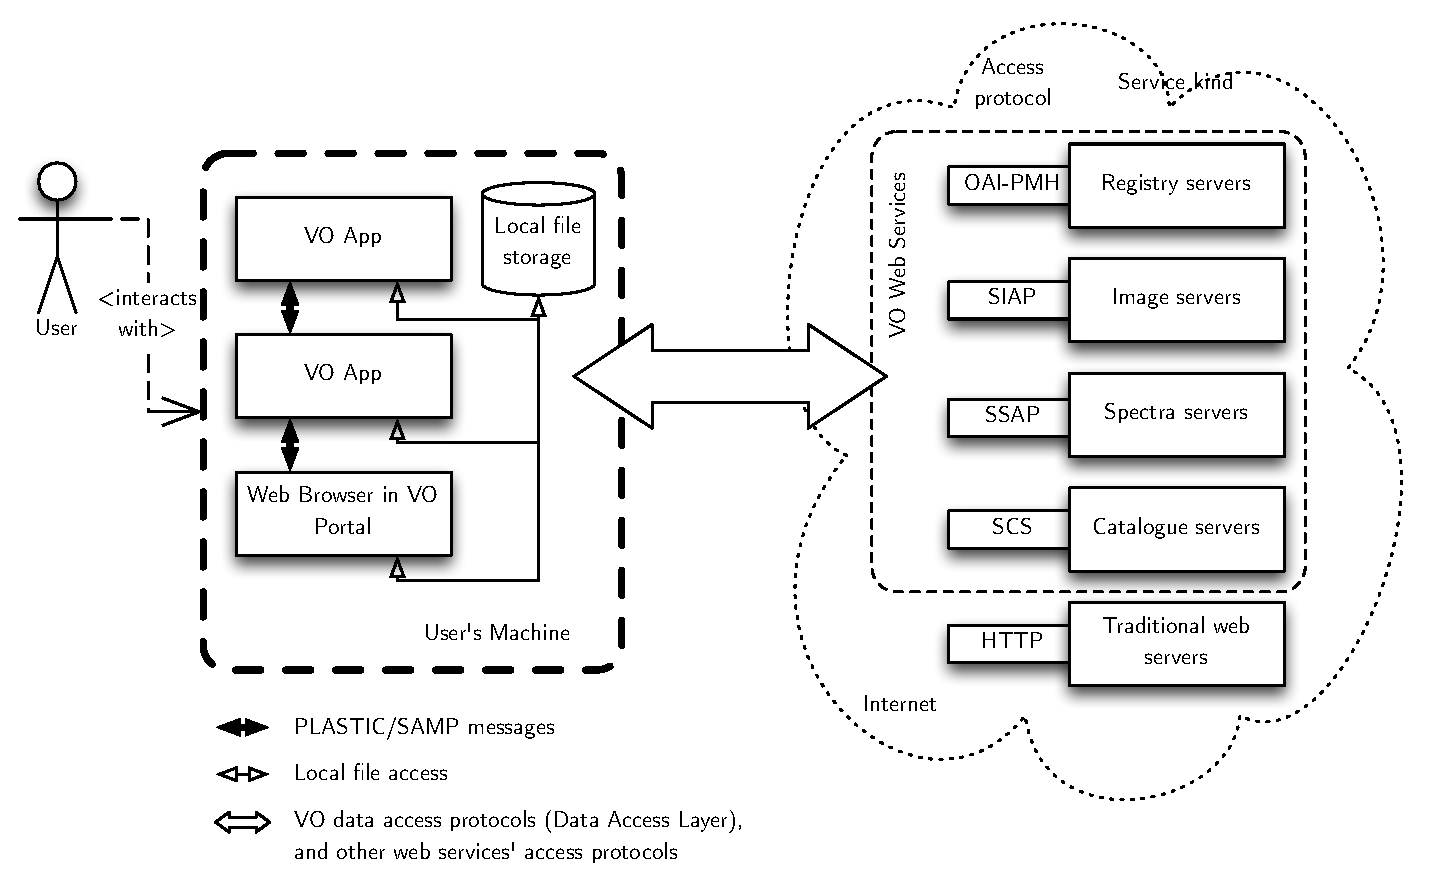
\includegraphics[width=\columnwidth]
				{fig/VOArchitectureFromUserPOV.pdf}
			\caption[User view of the VO]
			{
				High level VO architecture from the user's point of
				view. A user interacts with the VO via a variety of
				VO-aware, locally run applications, and accesses
				either locally archived files, or remote files,
				either via VO protocols or using a web browser to
				access a VO-enabled web portal. Users must only be
				aware of the different VO applications
				% \lourdesinline{VOapp no está definida}
				---VO app in the figure--- and/or VO portals of
				their interest, and that there exist interoperable
				image, spectra, and catalogue servers, transparently
				accessed from their toolset. They must also be
				aware that some VO applications can send messages
				and data between them, sending for instance data
				for analysis to some applications, and sending the
				received results to other applications for
				plotting. All the VO systems in the Internet
				---dotted cloud--- are indispensable for the
				operation of the VO, but are completely transparent
				to the user.
			}
			\label{fig:figUserPOV_VOArch}
		\end{figure}
		
		\invisiblenote{
			The VO architecture, as seen from the user point of
			view. Users can either access VO compatible files with
			VO-compliant tools, and use them more or less
			transparently in their workflow; or it could use a
			web-portal or a specific VO tool to explore VO datasets
			and retrieve those matching their criteria; or it could
			launch predefined VO-tasks on remote servers, which
			would bring VO compatible data back to the user.
		}
		
		 This can be better explained by means of an example.
		Imagine Alice is an astronomer who has already been
		introduced to the VO, and that she is searching for
		catalogues, images, and spectra on $\sigma$~Orionis, a
		star-forming region in the Orion belt.
		
		 She would fire up a tool such as the Aladin Sky Atlas, and
		use the search box to either specify the coordinates of the
		zone she is interested in, or would just write
		\texttt{sigma orionis}, and let Aladin query a name solver
		service, such as Sesame, to come up with the coordinates.
		
		 After having set the coordinates, Alice could set an
		angular radius for the search of interesting datasets,
		setting the separation for objects in the vicinity, or
		could just use the default radius. Aladin would ask
		different archives for both images and catalogues, laying
		catalogue data with coordinate information on top of the
		retrieved images, which can be composed from several bands.
		
		\begin{figure}[tbp]
			\centering
				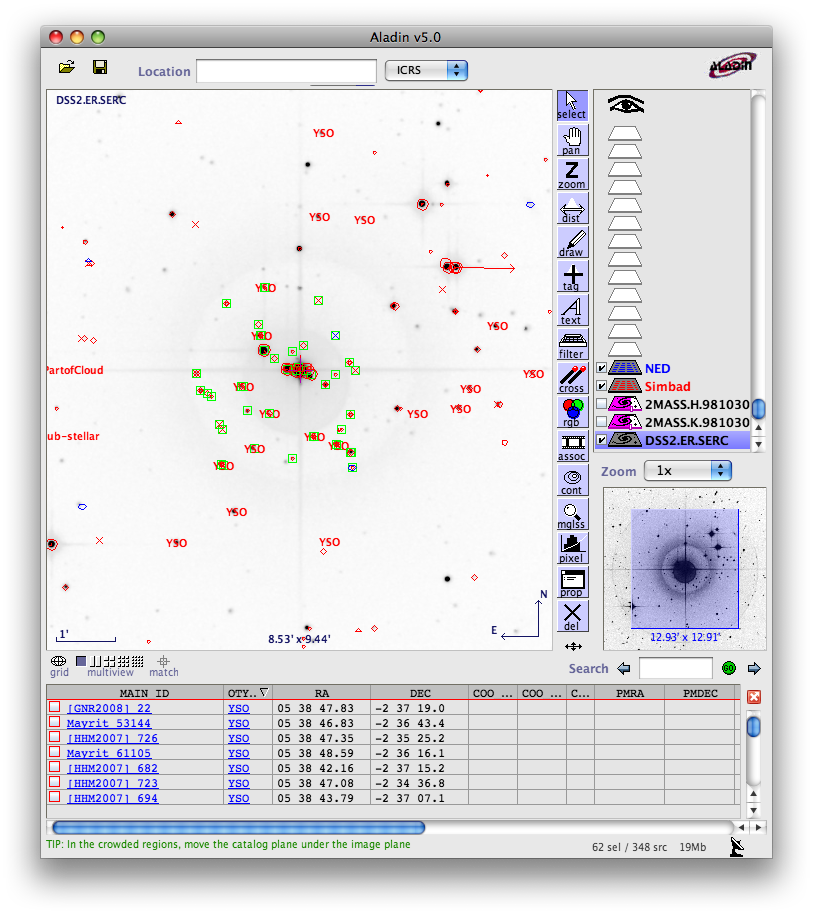
\includegraphics[width=\columnwidth]
				{fig/AladinSigmaOrionisDataSelection.png}
			\caption[Screenshot of the Aladin Sky Atlas]
			{
				Screenshot of the Aladin Sky Atlas: after having
				entered the coordinates for the $\sigma$~Orionis
				region in the search box on top of the window,
				Aladin has queried the Simbad and NED catalogues,
				together with the DSS2 server, and has overlaid
				catalogue objects on top of the DSS2 image.
				Besides, the astronomer has retrieved H-band and
				K-band images from the 2MASS survey, and has
				composed the three images by setting image
				transparencies. Besides, some data points of the
				central region have been selected, and are shown in
				the lower part of the window, sorted by the
				\texttt{OTYPE} (object type) column.
			}
			\label{fig:fig_AladinSigmaOrionisDataSelection}
		\end{figure}
		
		 She could, then, select catalogue data and send it to a
		table manipulation and plotting application, such as
		TOPCAT, to explore properties of the region.
		Figure~\ref{fig:fig_AladinSigmaOrionisDataSelection} shows
		what Alice's screen could look like while working with
		Aladin; figure~\ref{fig:fig_TopcatDatosSimbad}, instead,
		shows her computer's screen while using TOPCAT.
		
		\begin{figure}[tbp]
			\centering
				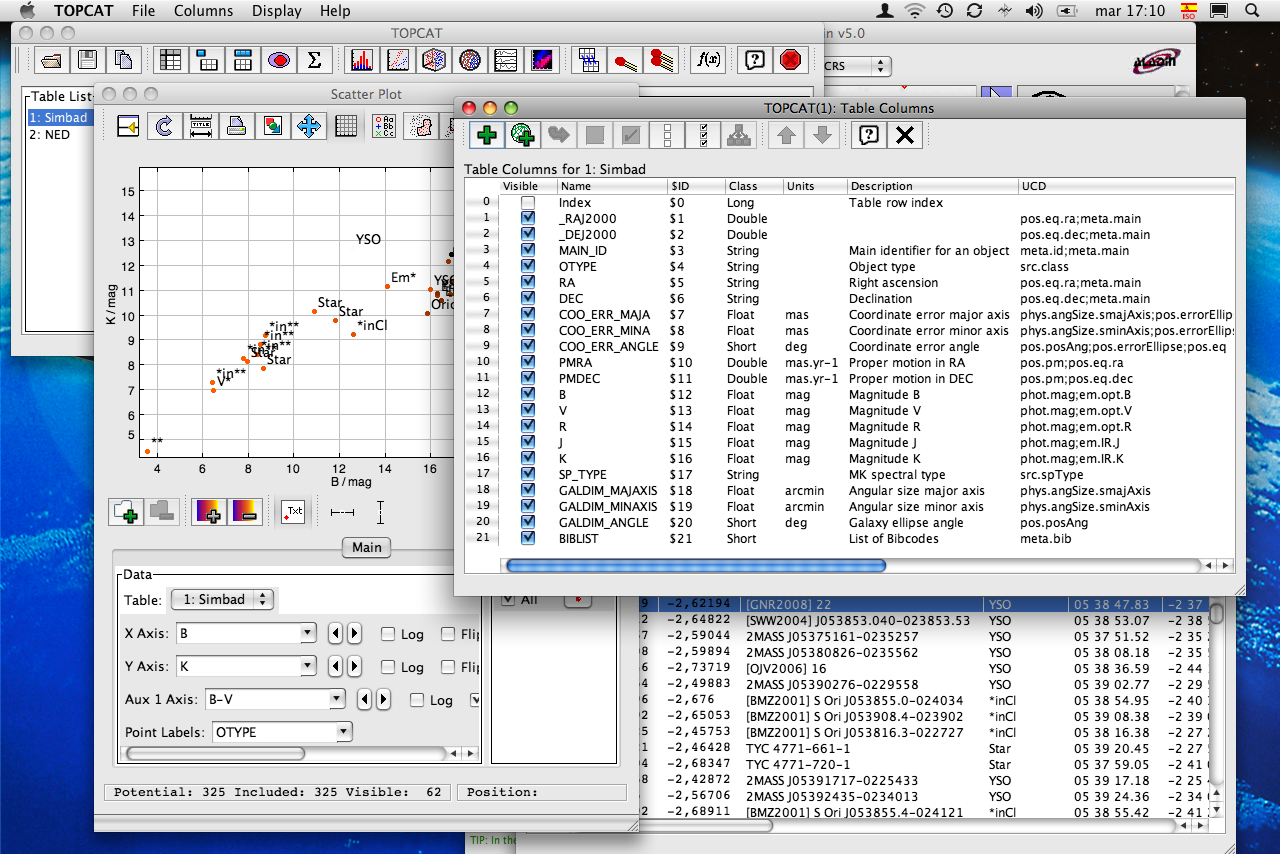
\includegraphics[width=\columnwidth]
				{fig/TopcatDatosSimbad.png}
			\caption[Screenshot of TOPCAT]
			{
				Screenshot of TOPCAT after having received two
				catalogues from Aladin via the PLASTIC VO messaging
				protocol. The windows shown, from left to right, and
				from top to bottom, are the main TOPCAT window,
				showing the two tables received from Aladin, which
				can be seen popping out to the right; a scatter
				plot of the $B$ magnitude against the $K$
				magnitude, using the $B-V$ color index for data
				point coloring, and with \texttt{OTYPE} as object
				label; the table column metadata, showing data
				types, units, description, and the UCD for of each
				column;
				% (the UCD is briefly described in 
				% section~\ref{sec:unified_content_descriptor_ucd})
				and the actual table data.
			}
			\label{fig:fig_TopcatDatosSimbad}
		\end{figure}
		
		 Another way to visualise the interaction of users with the
		VO is by means of a sequence diagram.
		Figure~\ref{fig:fig_VOClientSequenceDiagram} shows how
		users do not interact with VO services, they just interact
		with applications to provide object names, validate
		coordinates, and provide additional search criteria. VO
		applications are responsible of communicating with the
		different VO services (NameSolver, Registry, and data
		Services) on behalf of the user.
		
		% \lourdes{re-redactar párrafo anterior}
		
		\begin{figure}[tbp]
			\centering
				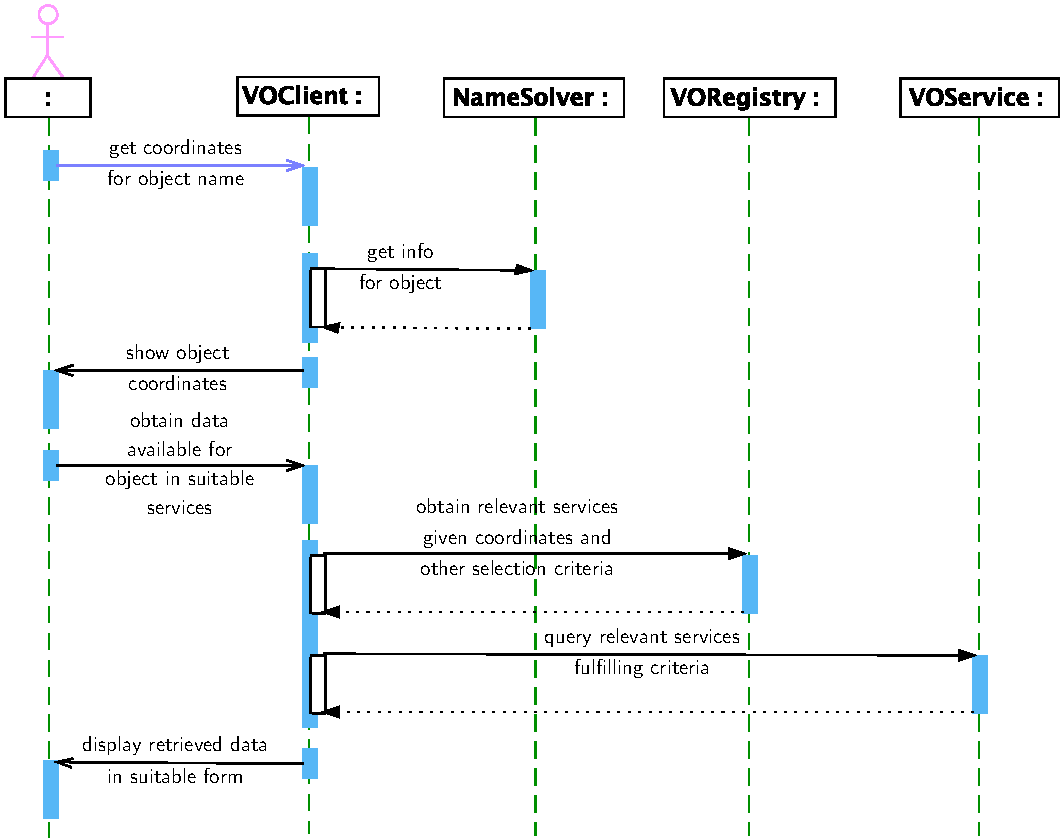
\includegraphics[width=\columnwidth]
				{fig/VOClientSequenceDiagram.pdf}
			\caption[Sequence diagram: User VO interaction]
			{
				UML sequence diagram of the user interaction with
				the VO. Users will typically use a VO client
				application to get information on particular
				objects of their interest. The user will first
				provide an object name, and the VO client will use
				an astronomical NameSolver to return celestial
				coordinates. With the coordinates, and some
				additional criteria, which might come from the
				application (a spectral analysis application will
				ask for spectral services; an image processing or
				manipulation package will ask for image services),
				or from additional criteria (wavelength, data
				quality, for instance) set by the user. Once the
				services are found, the application will query them
				(here only one such service query is shown), and
				the retrieved data will finally be provided to the
				user in a suitable form. This sequence diagram
				shows how user interaction with the VO is
				restricted to the use of VO application(s), while
				the orchestration of VO queries corresponds to the
				application.
			}
			\label{fig:fig_VOClientSequenceDiagram}
		\end{figure}
		
		For this user, the VO is just a set of software packages
		which can retrieve information from VO-enabled archives,
		and perform operations on such data, and on local data. The
		main differences with the way she used to work are:
		
		\begin{itemize}
			\item She uses spatial indexing on the data. Spatial
			selection goes first, archive, instrument, and
			wavelength selection are optionally performed in the
			next stage.
			
			 \item She does not have to know how many different
			archives might be of interest to her: within the VO,
			all archives containing data in the spatial zone of her
			interest will be queried. She can decide which data to
			finally download by looking at the archive metadata (to
			see if the wavelength range is appropriate or not, or
			who is responsible for the data quality), or at the
			particular dataset metadata (to learn specifics such as
			exposure time, observing configuration, and data
			quality flags).
			
			 \item She can combine the strengths of different tools
			by means of the VO messaging protocols.
			%\lourdesinline{presentar los local interop protocols.}
			
			 \item She can explore catalogues with higher
			confidence, because data columns are fully tagged with
			standard descriptors (UCDs, Unified Content
			Descriptors), which allow automated identification of
			those datasets.
		\end{itemize}
		
		In other words, she has transparent access to many archives
		not just from a single tool, but from any tool which is
		able to query the VO. In \emph{marketing} terms, any tool
		sporting a \emph{VO-compatible} badge.
		
		 However, if she wants to exploit the data she has just
		collected, for instance in order to perform cross-matching
		between sources, or to create different color diagrams, she
		needs to know how to find which data columns correspond to
		different astronomical or astrophysical concepts. In other
		words, she is concerned with data semantics.
		
		% However, the transparency to the user makes this view
		% miss the role of the VO as a standardisation force for
		% datasets, and also does not stress the power of common
		% semantics (the UCDs we have mentioned) between
		% archives, which allows for sensible comparison of
		% datasets.

	% subsection the_vo_from_the_point_of_view_of_the_user (end)

	\subsection{The VO from the application developer's point of view}
	% subsection % the_vo_for_the_application_developer (fold)
	\label{ssub:the_vo_for_the_application_developer}

		VO Developers view of the VO arises from what the VO offers
		for their applications. A VO-enabled application, be it
		brand new or upgraded, can be of two types: data centric or
		workflow centric. Some data centric applications can be
		scripted to be part of a workflow.
		
		 Data centric applications tend to be either data reduction
		applications or high level analysis applications which work
		on individual datasets at a time. For those applications,
		the VO is used for:
		
		\begin{description}
		
			\item[Finding out interesting datasets] That usually
		    means finding archives with data in the desired
		    wavelength range for certain positions of the sky.
			
			 \item[Retrieving candidate datasets] Candidate
		    datasets
			(be them images, spectra, data cubes)
			are downloaded
		    one by one, or as a package, to be individually
		    analysed in the local computer.
			
			 \item[Local processing] One by one processing of the
		    different datasets in order to obtain scientific grade
		    data products, such as chemical abundance, region
		    temperatures, ionisation states, stellar population
		    age, et cetera. Anything that is obtained from the
		    treatment of the light and the knowledge of the
		    physical process at hand.
		
		\end{description}

		 In this view of the VO, only a few benefits are added over
		the traditional astronomer's workflow, such as providing a
		single programmatic interface for all application to access
		all archives. That is, the VO provides a uniform data and
		metadata access, together with uniform data and metadata
		format to applications. Additionally, tools which implement
		VO messaging protocols allow the astronomer to use
		specialised tools for each task, while maintaining always
		the benefits of having each application connected to the
		VO.
		
		 On the other hand, workflow centric applications are
		applications which work with large datasets in large
		batches. For instance, from object types plus magnitudes in
		the 5 SDSS bands, photometric redshifts can be
		established\footnote{In fact, such processing is performed
		by the SDSS pipeline itself.}. Or data from different
		catalogues at different wavelengths can be cross-matched in
		order to find objects with particular properties which
		cannot be found through the original data of each
		individual dataset\footnote{If we have a catalogue of
		photometric magnitude measurements in $n$ bands per object,
		and combine it with $m$ additional photometric measurements
		in different bands, much more precise properties of those
		objects can be derived. As photometric redshift estimations
		make use of differences of magnitudes in as many bands as
		possible, their reliability depends on the number of pairs
		of magnitudes which can be built,
		$\begin{pmatrix}n\\2\end{pmatrix}$. But if we add $m$
		additional measurements, $\begin{pmatrix}n +
		m\\2\end{pmatrix}$ colours can be formed, and the relative
		increase in colours which can be formed is
		$\frac{(n+m)(n+m-1)}{n(n-1)}$, which is higher than the
		increase of just adding $m$ colours.}.
		
		 For those applications, the VO provides many more
		benefits: the access to archives is uniform, allowing
		simpler scripts, based around web services toolkits, to
		access all needed archives. Datasets are retrieved in a
		common format, and ready to analyse with XML tools.
		
		 Additionally, the VO community (in particular, the UK
		AstroGrid team\urlnote{http://www.astrogrid.org/}) has
		developed what is called the Common Execution Architecture
		(CEA)~\cite{Harrison:2005la}, a web-services wrapper for
		remote execution of tasks which can be called either with
		simple parameters (for instance, generating a synthetic
		spectrum from Kurucz models for stars with a given surface
		temperature, surface gravitational acceleration, and
		stellar type), or tasks which perform transformations on
		data in VOTable form (such as format transformations, or
		image generation from tabular data). As those tasks are
		exposed through a web services wrapper, users can get
		virtual data (data which was generated on the fly), or
		re-processed data, with the same kind of queries used for
		data retrieval.
		
		 In any case, the protocols that a VO application should
		implement are:

		\begin{description}
			\item[Object name queries] Many VO queries are
			spatially related, but for many sources there is a
			known source name, whose position is already well
			established. In those cases where the user wishes to
			query for other datasets near the source, being able to
			obtain the most recent coordinates, in different
			epochs, for a given object name, is one of the most
			important services in the VO. \invisiblenote{At the
			spatial level, it can be seen as similar to the
			internet Domain Name Solver services.} There are
			several services providing this target name to
			coordinates resolution, namely Sesame, the NASA
			Extragalactic Database (NED), and Simbad. However,
			Sesame is able to query both NED and Simbad, and is the
			primary service for name solving.
			
			 \newcommand{\cdssesamenote}[0]{ For instance, we can
			query Sesame about \emph{M31}, and we will learn that
			it is also known as \emph{Andromeda Nebula},
			\emph{Andromeda Galaxy}, or simply \emph{Andromeda}. In
			specific bands, it corresponds, for instance, with
			several strong infrared sources from the IRAS
			catalogue: \emph{IRAS~F00400+4059} and
			\emph{IRAS~00400+4059}. Sesame also returns object type
			information, and simply from querying Sesame we can
			learn that \emph{M31} is an active galaxy of
			\emph{LINER} type, with a morphology type of \emph{Sb}
			(a spiral galaxy without bars, with packed arms), and
			at a redshift (\emph{z}) of $-0.001004$, meaning that
			\emph{M31} is, in fact, blueshifted, getting nearer to
			the Milky Way at a rate of approximately $300
			\mathrm{km}/\mathrm{s}$.
			
			 The query which delivers all of this information, in
			XML format, is:
			
			 \noindent\url{\sesameurl}
		
			 See the CDS Developer's corner,
			\url{http://cdsweb.u-strasbg.fr/cdsws.gml}, for details
			on this and other services. }
			
			 An application querying Sesame must be able to parse
			not only the coordinates being provided, but also the
			different object aliases returned by the service, such
			as conventional names, coincidental sources at
			different wavelengths, morphology, redshift, and
			distance\footnote{\cdssesamenote}.
			
			 \item[Registry queries] Independently of the kind of
			VO services to be accessed, all applications must be
			able to query the VO Registry (or registries) so that
			they can look for specific services.
			
			 \item[Data access queries] Once we have coordinates to
			make our query (or queries), and the application (or
			the user) has selected entries in the registry that can
			provide useful datasets, the data access protocols
			relevant to the application (SCS, SIAP, SSAP, and in
			the future the TAP) have to be queried, and the
			returned data (in VOTABLE format) parsed.
			Appendix~\ref{cha:vo_protocols} is devoted to describe
			the interface to those services, and provides links to
			their complete specification.
			
			 \item[CEA services] If we want our application to take
			advantage of several remote VO services, such as those
			providing data transformation capabilities,
			mosaicing\footnote{Mosaicing is the non-trivial
			operation of overlaying several astronomical images,
			with embedded coordinates and resolution information,
			in order to provide a composition of the original
			images with a common resolution.}, signal processing,
			or many others running under the CEA, we must implement
			CEA services calls. The detailed description and
			specification of the CEA can be found
			in~\cite{Harrison:2005la}.
			
			 \item[Local messaging services] Optionally, the VO
			interoperability protocols for local data interchange
			and collaboration must be implemented. This allows a
			more modular development of VO tools, letting other
			applications to pre-process the data, and perform
			analysis in different ones.
		\end{description}

		In addition, as VO particular data formats are XML-based,
		XML manipulation toolkits are needed in order to build and
		interpret VO data, together with FITS processing libraries
		for applications which must have access to the actual data.

		\begin{figure}[tbhp]
			\centering
				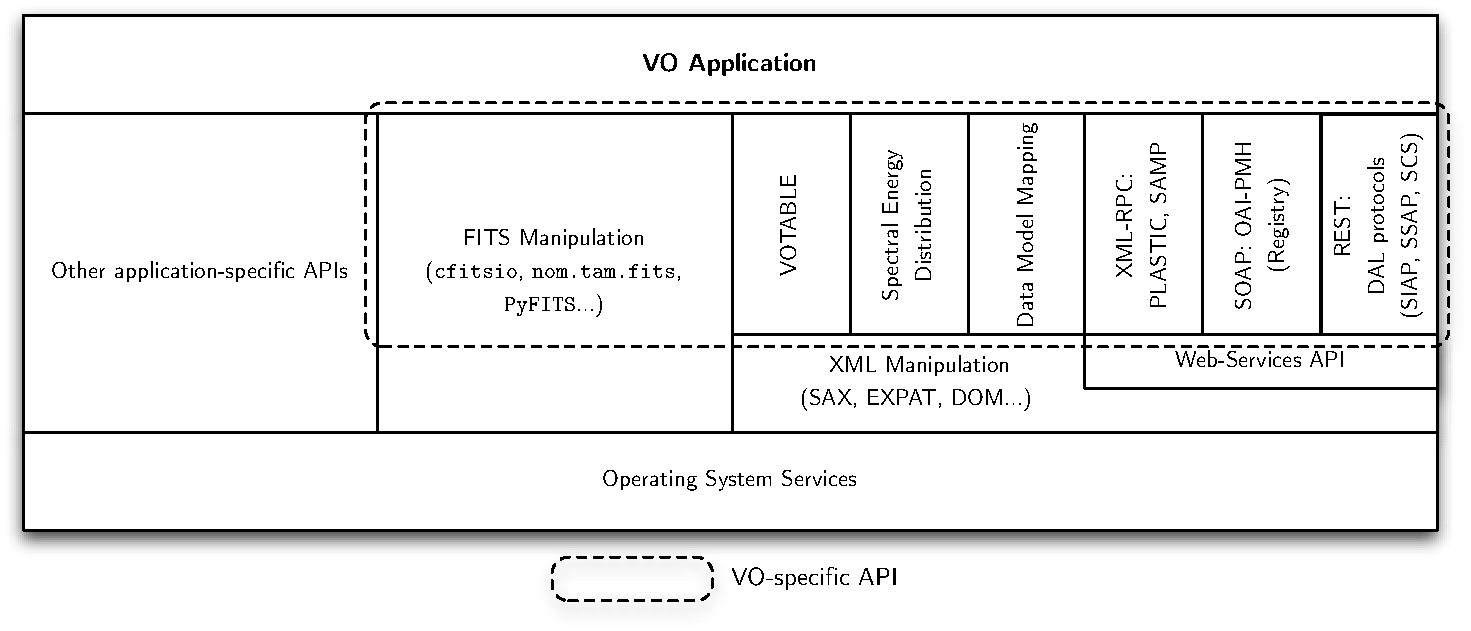
\includegraphics[width=\columnwidth]
				{fig/VOAPIStack.pdf}
			\caption[Application view of the VO]{
				The VO as seen from an application (developer)
				point of view. Applications trying to make use of
				the VO use web services technologies, such as REST
				queries, SOAP queries, or XML-RPC messages.
				Web-services calls require XML manipulation
				toolsets, which are also used to create, manipulate,
				and extract information from VOTables, the Spectral
				Energy Distribution XML representation, or
				different data model mappings. Finally, VOTABLEs
				can point to FITS files, and applications which
				manipulate scientific data must be able not only to
				read data from VOTables, but directly from FITS
				files. The VO specific part can be found in the
				dashed rounded rectangle, while the rest
				corresponds to either general APIs, or
				application-specific APIs.
			}
			\label{fig:fig_VOAPIStack}
		\end{figure}

		From the list above, it can be seen that the VO application
		interface for programmers (VO API) consists, then, of
		several more or less independent blocks, as shown in
		figure~\ref{fig:fig_VOAPIStack}.

		% We describe this programmatic interface to the VO with much
        % more detail in chapter~\ref{cha:voapi}.

		Let us imagine Bruce is an astronomical software developer.
		He has been creating astronomical software packages before
		the VO concept, and each time a new interesting archive
		appeared, he had to modify his application to perform the
		following tasks, every single time, without being able to
		reuse any code:

		\begin{description}
			\item[Service query] A new service query form, button,
			or other kind of user interactivity had to be added.
			
			 \item[Data access protocol] The query had to be
			implemented by encoding the service URL, service kind,
			and query parameters. Additionally, if the archive
			returns data in a particular format, a parser has to be
			implemented. % \lourdesinline{re-redactar}
			
			 \item[Data translation] The response data comes
			usually in a way that it is specific for the
			archive/service being queried, and must be translated
			into the data model of the querying application.
		\end{description}

		However, all steps above are common for all VO services
		providing the same kind of data (catalogues, images,
		spectra), with the addition of the Registry query step
		needed to find out all services providing that kind of
		data, which again has to be implemented only once.
		
		 It must be noticed that once the data are in the internal
		data model of the application, it does not matter which was
		the origin of a particular data set (except for documenting
		its provenance), and that is the way VO data can
		interoperate with non-VO data. An example of application
		mixing VO with non-VO data is Aladin: originally Aladin
		queried different non-VO services, and all VO-services were
		added as just one additional data source for Aladin.


	%	The VO as an Application Programming Interface. An
	%	application making use of the VO can see the different
	%	services it provides as a VO API. The different parts of
	%	the API are built on top of web-services client frameworks,
	%	and XML and FITS manipulation toolkits.
	%	
	%	 In fact, the AstroRuntime, from AstroGrid, provides such
	%	an API to the VO to allow XML-RPC enabled languages to
	%	programmatically access VO facilities, with an additional,
	%	more direct layer for Java applications through Java-RMI.


	% subsection % the_vo_for_the_application_developer (end)

	\subsection{The VO from the service developer's point of view}
	% the_vo_from_the_point_of_view_of_the_service_developer (fold)
	\label{ssub:the_vo_from_the_point_of_view_of_the_service_developer}

		For Bruce, then, the VO is technically rather simple
		(compared with the archive access and interface operations
		already in place in the archive): the services have to
		provide access to existing datasets through a web-services
		interface (most of the time, REST-ful services are used for
		the VO, except for VO Registry services, which use SOAP
		queries).
		
		 However, the hardest part for VO-services developers is
		the interfacing between the actual data being stored, and
		the VO data formats, which also include VO semantics. This
		is achieved by means of a systematic mapping between stored
		data and data models.
		
		 In particular a VO service needs to provide:

		\begin{description}
			\item[VO Service Endpoint(s)]
			% \lourdesinline{Explicar DAL, explicar endpoint}
			A service provider must provide one or more VO services
			(delivering images, spectra, or catalogue data). Each
			different service must provide an URL for accessing it,
			the endpoint. This URL is used to build VO queries by
			adding parameters to it. Different services, in the
			sense that the data they provide corresponds to a
			different scientific data product, need to provide
			different endpoints.
			
			 \item[DAL Parser and Query Mechanism] The service
			endpoint parameters have to be parsed, converted into a
			query for the internal database (or any other data
			access and filtering mechanism), and results obtained.
			In short, the service must comply with the interfaces
			described in appendix~\ref{cha:vo_protocols}.
			
			 \item[VOTable generation mechanism] Once the query has
			returned results, these must be returned into the
			VOTable format. This includes not only the building of
			the main tags, which can be considered a wrapper for a
			tabular result, but also the assignment of semantic
			attributes such as \texttt{ucd}s and \texttt{utype}s
			from data model mappings.
			
			 \item[Data Model Mapper] The VOTable generation
			mechanism, and the DAL Parser, need a mapping between
			the data stored in the database and the data model for
			the kind of observation being performed. This mapping
			is used for the filling of the already mentioned
			semantic attributes.
			
			 \item[CEA wrapper] A service which provides computing
			services in the VO environment has to comply with the
			CEA. A computing service which was not built for the VO
			can integrate into the CEA infrastructure by
			encapsulating it into a CEA intermediate service
			(wrapper).
			% \lourdesinline{Explicar wrapper.}
		\end{description}

		Other task to be eventually performed by the VO Service
		developer is the endpoint registration. Even when the VO
		Service can be used as long as its endpoint is known by any
		other tool (be it a simple command-line script, or a
		complete application), new services can only be discovered
		by tools if they are registered in a VO Registry.

	% subsection
	% the_vo_from_the_point_of_view_of_the_service_developer (end)

% section the_vo_from_the_point_of_view_of_different_actors (end)
	
	\section{Precedents to the VO} % (fold)
	\label{sec:precedents_to_the_vo}
		
		Due to the purely scientific, non-commercial nature of astrophysical
data, public access to them has always been the norm. With the
connection of most educational and research institutions to the
Internet, the first primitive online archives were born. One of the
first was that of the International Ultraviolet Explorer (IUE), which
was made available to the public in 1985. As the World Wide Web did not
exist yet at that time, astronomers had to login to remote servers from
which the data were downloaded through the File Transfer Protocol
(FTP).

Apart from the data from observations themselves, articles and other
publications on astronomical objects were also of great value, and
during the \emph{Astronomy from large databases}
conference~\cite{1988afld.book.....M}, held in 1987, a proposal was
made for the design and operation of a system to compile all
astronomical publications, the SAO/NASA Astrophysics Data System (ADS).
A prototype was built in 1990, with the system being released to the
public in early 1993~\cite{1993ASPC...52..132K}. The system was made
possible thanks to the collaboration of the publishing journals.

Simultaneously, systems like the Simbad Astronomical
Database\urlnote{http://simbad.u-strasbg.fr/simbad/}~\cite{
2000A&AS..143....9W} (an online database hosted by the Centre de Donées
Astronomiques de Strasbourg, CDS), or the NASA/IPAC Extragalactic
Database\urlnote{http://nedwww.ipac.caltech.edu/}~\cite{
1992ASPC...25...47M} (NED) contained data with diverse information on
observed astrophysical objects, which were compiled, maintained and
published online by the respective large scale astronomical data
centres.

\newcommand{\adsbibcodeurl}[0]
{http://doc.adsabs.harvard.edu/abs_doc/help_pages/bibcodes.html}
As all of these initiative had grown independently, the were developed
with different considerations in mind, and were not coordinated.
However, the possibility of joining publications available at the ADS,
and the Simbad/NED databases, allowed astronomers to have access to
publications on the objects of their interest, or to access more data
in those databases from the corresponding literature. The joint
ADS/NED/Simbad effort was called URANIA~\cite{1996AAS...189.0603B}, and
is one of the first joint initiatives for data service interoperability
in astronomy. The main product of that agreement is the
\emph{bibcode}\urlnote{\adsbibcodeurl}, a unique identifier of
publications which encodes details on the publication date, publication
kind, and/or journal, and author\footnote{When astronomers upload data related to a particular publication to the NED or Simbad services, or that data is gathered from the publication, the bibcode allows the cross-identification of sources and publications.}.

\newcommand{\vizierurl}[0]
{http://webviz.u-strasbg.fr/viz-bin/VizieR}
Outside the URANIA project, the
INES\urlnote{http://sdc.laeff.inta.es/ines/} (IUE Newly Extracted
Spectra)~\cite{1999A&AS..139..183R} archive, holding reprocessed IUE
observations, represents the first instance of interoperability between
two completely different astrophysical services: one holding spectral
information (INES), the other keeping bibliographical references (ADS).
It was possible to access the information available in ADS for a
particular object from the INES archive, and from the ADS the INES
spectra used for a particular article could be accessed. Other service
linked to the ADS through bibcodes is the VizieR\urlnote{\vizierurl}
service for Astronomical Catalogues~\cite{2000A&AS..143...23O}.

Another important milestone in the development of online, interoperable
archives was the NASA multi-mission archive initiative, which tried to
provide a common archival infrastructure across different space-borne
missions. Three portals were finally created:
MAST\urlnote{http://archive.stsci.edu/} (Multi-mission Archive at Space
Telescope)~\cite{1999AAS...194.8302I}, mainly for optical-ultraviolet
observations\footnote{VLA FIRST images are also available through
MAST.}; IRSA\urlnote{http://irsa.ipac.caltech.edu/} (InfraRed Science
Archive)~\cite{2000AAS...19711610B}, for the infrared; and
HEASARC\urlnote{http://heasarc.gsfc.nasa.gov/} (High Energy
Astrophysics Science Archive Research
Center)~\cite{1994BAAS...26..995R} for high-energy (X-rays, gamma rays)
astrophysical observations. These portals allowed for the first time a
unified view of data from widely different provenance under the same
query interface. MAST also provided some applications for data
visualisation across mission, such as the
COPLOT\urlnote{http://archive.stsci.edu/mast_coplot.html} tool.
However, data products from each mission were, still, quite different.

Finally, regarding the use of applications in order to combine and
manipulate data from different services, one of the first examples
prior to the VO development is the Aladin Sky Atlas. Initially, Aladin
was only able to access CDS-based catalogues and images, which were
accessed through custom built, Aladin-specific protocols. However,
Aladin helped in making developers and astronomers realise that any
other system which shared the data access and data description
protocols would allow either to improve Aladin, by allowing it to
access more datasets, or more easily recreate Aladin-like functionality, without the need of being a data and service provider.
		
		\invisiblenote
		{The VO infrastructure has taken advantage of already in
		place systems. The main precedents are:
		
		\begin{description}
			\item[The NASA/IPAC Extragalactic Database] The
			NED\urlnote{http://nedwww.ipac.caltech.edu/}~\cite{
			1992ASPC...25...47M} (service acronym), provides online
			all different catalogues of extragalactic objects ever
			published in astronomy. It allows users to perform
			\emph{conesearchs} for data centred on a particular
			position, and below a certain angular distance, and the
			results provide the main object positional properties:
			sky coordinates, distance, relative velocity, object
			type, morphological classification, et cetera; it also
			provides many other observational parameters, such as
			galactic extinction, absolute magnitudes, et cetera.
			
			 \item[The Simbad Astronomical Database]
			Simbad\urlnote{http://simbad.u-strasbg.fr/simbad/}~\cite{
			2000A&AS..143....9W} is an online database hosted by
			the Centre de Donées Astronomiques de Strasbourg (CDS),
			also providing data on different objects outside of our
			solar system, and thus includes galactic objects. The
			two databases have a non-empty intersection, but none
			is a subset of the other.
			
			\newcommand{\vizierurl}[0]
			{http://webviz.u-strasbg.fr/viz-bin/VizieR}
			\item[The
			VizieR service for Astronomical Catalogues]
			VizieR\urlnote{\vizierurl}~\cite{2000A&AS..143...23O}
			is a compilation of all published astronomical
			catalogues, classified by waveband coverage, space
			mission if applicable, and/or astrophysical subject.
			Many astrophysical journals automatically make
			available in VizieR positional tables in published
			articles, and the data is linked to the publication via
			the \emph{bibcode} of the Astrophysics Data System
			(ADS).
			
			\newcommand{\adsbibcodeurl}[0]
	   {http://doc.adsabs.harvard.edu/abs_doc/help_pages/bibcodes.html}
			\item[The SAO/NASA Astrophysics Data System] The
			ADS\urlnote{http://www.adsabs.harvard.edu/}~\cite{
			2000A&AS..143...41K} is an online da\-ta\-base
			containing all bibliographic entries in the fields of
			Physics and Astrophysics. Entries are proposed by
			different journal and book publishers, but are also
			collected from online e-print archives such as the
			arXiv\urlnote{http://arXiv.org/}. Publications are
			uniquely identified by a structured code, the
			\emph{bibcode}\urlnote{\adsbibcodeurl}, which contains
			details on the publication date, publication kind,
			and/or journal, and enough data for unique
			identification or journal articles. The entries are
			linked with online versions of the articles, if
			available, and can be searched by author, words in
			title or abstract, publication dates, et cetera. VizieR
			catalogue entries are also considered publications by
			the ADS, with their own \emph{bibcode}.
		\end{description}
	
		These facilities have been federated and linked by means of
		the \emph{bibcode}, which allows for the retrieval of
		publications on any object in Simbad or NED, or for the
		objects whose data is found in VizieR.
		
		 And many observatories, specially space-borne ones, have
		had online archives from little time after the opening of
		the Internet and the World Wide Web.
		
		 However, all of these services have their own, completely
		different form-based interfaces, and even when they have
		started to provide cleaner web-services interfaces, users
		need to support different query protocols for each service,
		until the VO provided service unification and
		interoperability templates.
		}
	% section precedents_to_the_vo (end)

	\section{Comparable activities in other disciplines} % (fold)
	\label{sec:comparable_activities_in_other_disciplines}
	
	We will conclude our introduction of the VO with a selection of
	other e-science activities which are similar in scope to the
	Virtual Observatory, but belong to different scientific fields,
	or have a different technology base: the data storage support
	of data grids, Geographical Information Systems, and the
	Bioinformatics Harvester.
	
	\subsection{Data grids} % (fold)
	\label{sub:data_grids}
	
		In e-Science talks, grid technologies tend to come up first
		and forefront. It is very usual for national e-Science
		initiatives in European countries to be represented by the
		National Grid Initiatives, as if e-Science could only be
		performed via grid technologies. It is true that grid
		middleware provides tools to implement much of VO core
		functionality, but at the cost of a greater complexity, and
		greater demands on client systems.
		
		 The definition of grid computing by Ian Foster as \emph{a
		hardware and software infrastructure that provides
		dependable, consistent, pervasive, and inexpensive access to
		high-end computational
		capabilities}~\cite{1999gbnc.book.....F} is just one part
		of the Virtual Observatory.
		
		 But computation is just a fraction of the VO. In fact, the
		VO can be more closely identified with a \emph{data
		grid}~\cite{Chervenak:2001rr}: an extension of the grid
		protocols in order to create a standard for distributed
		data storage, data identification, and metadata management
		which can integrate archives from different disciplines.
		
		 In the VO, the \emph{data grid} exists via the data access
		protocols, and the standardisation of metadata. A version
		of the VO can exist implemented on top of grid protocols,
		but web-services technology was chosen instead in order to
		minimise the cost of entry for participant
		institutions/research groups: web-services technology is
		easier to implement and deploy, both for servers and
		specially for clients, and it was very important to be able
		to have a productive VO that could engage the community.
		
		 In the future, however, the VO can move more towards a
		grid technology foundation, when the computing needs
		overcome the data needs, and the VO metadata standards are
		complete. In the meantime, VO protocols are as technology
		agnostic as possible. For instance, the IVOA is working in
		a distributed file system for VO tools, reminiscent of grid
		data storage pools, with VO specific metadata and
		implementation independent (it can use WebDAV, NFS,
		GridFTP, or any other supporting protocol), called
		VOSpace~\cite{2008vospcivoav1013G}.
	% subsection data_grids (end)
	
	\subsection{Geographical Information Systems} % (fold)
	\label{sub:geographical_information_systems}
	
		There are many similarities between the VO and 
		Geographical Information Systems (GIS):
	
		\begin{description}
			\item[Coordinate system based] Both for GIS and the VO,
			coordinates are one of the main indices on data.
			Finding data nearby a particular coordinate is also a
			common feature, and the retrieval of nearby candidates
			cannot be based on floating point differences, as it
			would become computationally costly. The solution for
			fast operation of coordinate-based data retrieval is
			the hierarchical partitioning of the search space
			using, for instance, techniques such as the
			Hierarchical Triangular Mesh~\cite{2001misk.conf..631K}
			or the Quad Tree Cube~\cite{2006ASPC..351..735K}.
			
			 \item[Object to coordinates resolution] Also common to
			both problem domains is the need to obtain coordinates
			for a particular object whose only known property is
			the name. In astronomy such needs are typically handled
			by the Simbad or NED services, while different GIS
			systems will use different local or remote databases
			for obtaining the coordinates.
			
			 \item[Use of metadata] GIS objects are primarily
			graphs\footnote{In the mathematical sense: a
			set of directed connections between sets of nodes.}
			with geographical coordinates attached to both
			connections and nodes. But those curves represent
			roads, buildings, water and gas distribution pipes,
			agricultural plantations, et cetera, and each object
			kind has its own set of metadata, in the same way VO
			data uses metadata to establish object kind, and
			information kind.
		\end{description} 
	
		The main difference between the VO and GIS systems is that
		for the VO there is a strong standardisation force
		mandating which data formats to use, and there is usually
		no restriction in data usage\footnote{After all,
		astrophysical data tend not to be of immediate value for
		entrepreneurial use.}, and interoperation and networking is
		a key concept in system design, while it is not so for GIS.
		
		 However, some GIS systems such as Google
		Earth\urlnote{http://earth.google.com/} have started to
		show the potential of having a common geographical
		description format combined with the distributed dataset
		creation and distribution: GIS data, both images and object
		catalogues with metadata can be updated on the data server,
		and all clients access updated data from then on.
		
		 It is remarkable in this context that Google Earth has
		evolved to include Google Sky, which demonstrates the
		similar nature of GIS and VO systems when the distributed,
		interoperable data access is taken into account.
	
	% subsection geographical_information_systems (end)
		
	\subsection{Bioinformatic Harvester} % (fold)
	\label{sub:genbank}
	
		The Bioinformatic
		Harvester\urlnote{http://harvester.fzk.de/harvester/}
		(BioH) is a bioinformatic meta search engine at KIT
		Karlsruhe Institute of Technology for genes and
		protein-associated information. It queries data from more
		than 35 bioinformatic sites, which allows for searches in
		the genome and proteins of several animals of the most
		important sequenced animals ---among them humans, rats, or
		the drosophila (fruit fly)--- or on the complete
		collection.
		
		 The similarities with the VO lie in the distributed nature
		of the integrated systems, but the similarities end there:
		
		\begin{itemize}
			\item the BioH does not use a unified, standardised
			protocol for harvesting the data available in the
			different resources; instead, it uses a custom built
			harvesting engine for each collection.
			
			 \item there is only one entry point to the Harvester,
			and there is no public service access entry point for
			external applications.
		\end{itemize}
		
		 We can see the BioH as bioinformatic equivalent of the
		state of affairs in astronomy prior to the VO: similar to
		the joint ADS and VizieR systems.
	
	%GenBank\urlnote{http://www.ncbi.nlm.nih.gov/Genbank/} is the
	%NIH genetic sequence database, an annotated collection of all
	%publicly available DNA sequences. It contains approximately 86
	%thousand million bases in almost 83 million sequence records in
	%the traditional GenBank divisions, while more than 100 thousand
	%million bases on 27 million sequence records are held in the
	%WGS (large genome sequencing projects) division.
	%
	% The main connection point with the VO is that it is a public
	%driven effort which is central to a particular community
	%(astronomers for the VO, geneticists for the GenBank). However,
	%the GenBank is quite opposite to the VO in many aspects:
	
	
	% subsection genbank (end)
	
	% section comparable_activities_in_other_disciplines (end)
	
	\section{Status of the VO} % (fold)
	\label{sec:status_of_the_vo}
		
		As we have said, the VO initiatives were conceived around
		2000, and first prototypes built around 2002. Even
		when some parts of the VO are still being built ---being
		the IVOA Table Access Protocol (TAP) one of the salient
		examples of \emph{in progress} infrastructure---, and
		some of them being subject to changes (the Image and
		Spectral Access protocols are being reviewed), many of
		the tools are mature enough as to produce scientific
		results beyond what was possible prior to the VO.
		
		In particular, the first paper on VO-enabled science
		was published by Paolo Padovani in
		2004~\cite{2004AaA...424..545P}, and reported on the
		discovery of faint, obscured quasars with Virtual
		Observatory tools. However, more than half of all
		VO-enabled scientific
		papers\urlnote{http://www.euro-vo.org/pub/fc/papers.html}
		have been published since 2007 and onwards, while
		more than 90 percent of papers were published after 2006,
		which indicates a shift toward the maturity of the VO
		infrastructure and tools.
		
		\newcommand{\votableoneohurl}
	{http://www.ivoa.net/Documents/PR/VOTable/VOTable-20031017.html}
		\newcommand{\siaoneohwdurl}
		{http://www.ivoa.net/Documents/cover/SIA-20040524.html}
		\newcommand{\ssaoneoneprurl}
		{http://www.ivoa.net/Documents/cover/SSA-20070604.html}
		This can be easily correlated with the development of IVOA
		standards: the first IVOA Recommendation of the VOTable
		dates from October 2003\urlnote{\votableoneohurl}; the
		first agreed working draft for the Simple Image Access
		protocol was published in 2004\urlnote{\siaoneohwdurl}; the
		first ConeSearch services were available soon after that,
		with the ConeSearch specification being published in 2006;
		the Simple Spectral Access protocol, finally, was only
		proposed as a recommendation in
		2007\urlnote{\ssaoneoneprurl}, and prior to that only
		prototype spectral services, reusing the Image Access
		protocol, existed.
		
		It is interesting to mention that one of the national
		VO initiatives pushing the most towards the development of
		VO scientific tools is the SVO, as more than half of VO
		papers have been published by SVO-related groups.
		
		%\todo{\textbf{Enrique}, ¿puedes confirmar esto?}
		
		In the IVOA InterOp meeting of Baltimore (October, 2008),
		the former IVOA Chair, Dave de Young, proclaimed the VO
		had entered the operational status, where all infrastructure
		is mostly put into place, and science is routinely possible
		with existing tools.
		
		In this thesis, we will try to help in bringing radio
		astronomical archives and tools to that operational stage.
		
	% section status_of_the_vo (end)
	
	
	
%	\section{Current problems of the VO} % (fold)
%	\label{sec:current_problems_of_the_vo}
%
%		Even now that the IVOA and the VO have been declared as
%		reaching operational status at the IVOA Fall InterOp of
%		Baltimore in 2008, many issues are still open,
%		or are of further concern:
%		
%		\begin{description}
%			\item[Registries contain lots of useless entries] The
%			minimum mandatory metadata for a resource entry is mandated
%			by the Dublin Core metadata, but it is not enough for many
%			applications. In addition, some registry entries for VO
%			services are outdated, and link to non-existing servers.
%			Automated checks of the validity of registry entries are
%			useful, but manual purging of non-useful entries should
%			decrease the number of entries, and increase the usefulness
%			of the registry as a whole. In any case, users and/or VO
%			tool developers need to take this into account.
%			
%			\item[label] description
%			\item[Many tools have not made the transition the VO]
%			Many astronomical tools
%		\end{description}
%
%	% section current_problems_of_the_vo (end)

% chapter intro_vo (end)